\documentclass[10pt]{article}
\usepackage[utf8]{inputenc}
\usepackage[T1]{fontenc}
\usepackage{amsmath}
\usepackage{amsfonts}
\usepackage{amssymb}
\usepackage[version=4]{mhchem}
\usepackage{stmaryrd}
\usepackage{hyperref}
\hypersetup{colorlinks=true, linkcolor=blue, filecolor=magenta, urlcolor=cyan,}
\urlstyle{same}
\usepackage{caption}
\usepackage{graphicx}
\usepackage[export]{adjustbox}
\graphicspath{ {./images/} }

\title{Pulsar Survey Forecasts and Strategies for the DSA-2000 }

\author{Version: 1.3\\
Version date: 2025-09-22\\
Original date: 2025-08-06\\
Controlled document: No\\
WBS Level 2: RCF\\
Document type: OTH}
\date{}


%New command to display footnote whose markers will always be hidden
\let\svthefootnote\thefootnote
\newcommand\blfootnotetext[1]{%
  \let\thefootnote\relax\footnote{#1}%
  \addtocounter{footnote}{-1}%
  \let\thefootnote\svthefootnote%
}

%Overriding the \footnotetext command to hide the marker if its value is `0`
\let\svfootnotetext\footnotetext
\renewcommand\footnotetext[2][?]{%
  \if\relax#1\relax%
    \ifnum\value{footnote}=0\blfootnotetext{#2}\else\svfootnotetext{#2}\fi%
  \else%
    \if?#1\ifnum\value{footnote}=0\blfootnotetext{#2}\else\svfootnotetext{#2}\fi%
    \else\svfootnotetext[#1]{#2}\fi%
  \fi
}

\begin{document}
\maketitle
\captionsetup{singlelinecheck=false}
DSA-2000 Document No. 00151

\begin{center}
\begin{tabular}{|l|l|l|l|}
\hline
 & Name & Signature (PDF) & Date \\
\hline
PI &  &  &  \\
\hline
Subsystem Lead &  &  &  \\
\hline
Project Engineer &  &  &  \\
\hline
Project Manager &  &  &  \\
\hline
\end{tabular}
\end{center}

\begin{center}
\begin{tabular}{|c|c|c|}
\hline
 & DSA-2000 Document No. 00151 & Version: 1.3 \\
\(\square S \wedge-20 \mathrm{O}\) & \begin{tabular}{c}
Pulsar Survey Forecasts and Strategies for the DSA- \\
2000 \\
\end{tabular} & \begin{tabular}{c}
Date: \(2025-09-22\) \\
Page: \(2 / 19\) \\
\end{tabular} \\
\hline
\end{tabular}
\end{center}

Revision History

\begin{center}
\begin{tabular}{|l|l|l|l|l|}
\hline
Ver. & Date & Sections Affected & Reasons / Remarks & Author(s) \\
\hline
1 & 2025-08-06 & All & Original & Myles Sherman \\
\hline
1.1 & 2025-08-08 & Abstract, 1, 3 & SEFD for the new array & Myles Sherman \\
\hline
1.2 & 2025-08-18 & Abstract, 1, 3 & SEFD for the new array design corrected to 1.6 Jy [minor] Added a footnote regarding original gain estimate [minor] & Myles Sherman \\
\hline
1.3 & 2025-09-22 & 1 &  & Myles Sherman \\
\hline
\end{tabular}
\end{center}

\footnotetext{\({ }^{\text {a }}\) The original \(G=4.17 \mathrm{~K} /\) Jy estimate is conservative and assumes that an arbitrary fraction of baselines would be removed to reduce computation for the pulsar search (SEFD\~{}6 Jy). The current design now assumes that all baselines will be included, leading to a significant improvement in gain ( \(G=17.5 \mathrm{~K} / \mathrm{Jy}\) ) in addition to the effect of hardware updates.
}\begin{center}
\begin{tabular}{|c|c|c|}
\hline
 & DSA-2000 Document No. 00151 & Version: 1.3 \\
\(\square S \wedge-20 \mathrm{O}\) & \begin{tabular}{c}
Pulsar Survey Forecasts and Strategies for the DSA- \\
2000 \\
\end{tabular} & \begin{tabular}{c}
Date: 2025-09-22 \\
Page: \(3 / 19\) \\
\end{tabular} \\
\hline
\end{tabular}
\end{center}

\section*{Table of Contents}
1 Introduction ..... 4\\
2 DSA-2000 Pulsar Search Design ..... 5\\
3 Pulsar Detection Forecasts ..... 6\\
4 CASS Target Selection and Multi-Wavelength Cross-Matching ..... 8\\
5 Cadence, Follow-up, and Confirmation Strategy ..... 11\\
6 Conclusion ..... 14\\
7 Appendix: Modelling the Effective DSA-2000 Blind Search S/N Threshold ..... 14\\
8 References ..... 17

\footnotetext{\({ }^{\text {a }}\) The original \(G=4.17 \mathrm{~K} /\) Jy estimate is conservative and assumes that an arbitrary fraction of baselines would be removed to reduce computation for the pulsar search (SEFD\~{}6 Jy). The current design now assumes that all baselines will be included, leading to a significant improvement in gain ( \(G=17.5 \mathrm{~K} / \mathrm{Jy}\) ) in addition to the effect of hardware updates.
}\begin{center}
\begin{tabular}{|c|c|c|}
\hline
 & DSA-2000 Document No. 00151 & Version: 1.3 \\
\(\square S \wedge-20 \mathrm{O}\) & \begin{tabular}{c}
Pulsar Survey Forecasts and Strategies for the DSA- \\
2000 \\
\end{tabular} & \begin{tabular}{c}
Date: \(2025-09-22\) \\
Page: \(4 / 19\) \\
\end{tabular} \\
\hline
\end{tabular}
\end{center}

\begin{abstract}
With a comparable sensitivity to the Arecibo telescope and a \(10.6 \mathrm{deg}^{2}\) field of view \textbf{(may be inconsistent with the \(\sim 7.3\,\mathrm{deg}^2\) value at 1100 MHz stated later; if so, update for consistency)}, the Deep Synoptic Array (DSA-2000) has the potential to dramatically improve the census of Fast Time Domain (FTD) radio transients through a dedicated search. The unique instrument design motivates consideration of unique pulsar search strategies. In this memo, we present forecasts for the number of pulsars detectable by the DSA-2000, examine the prospects for continuum source targeting, and discuss how the unique cadenced search strategy can be leveraged for pulsar search follow-up. The \href{http://PSRPop.py}{PSRPop.py} population synthesis software is used to generate a model pulsar population, and the sensitivity of the DSA2000's initial design \(T_{s y s} \approx 25 \mathrm{~K}\) used to predict the number that will be detectable. Multiwavelength catalogs and images from the COSMOS deep field are used to model a theoretical continuum source cross-matching process which could be used for a real-time targeted pulsar search with the DSA-2000. This strategy will rely on unique synergies with future deep all-sky radio and optical catalogs from SPHERE-X, Roman and Euclid telescopes. We predict the DSA-2000 will detect 3000 millisecond pulsars and 20000 slow pulsars by incorporating data from the first epoch of the Continuum All Sky Survey (CASS) into the periodicity search. The DSA-2000 pulsar search will increase the known population by a factor of 7, driving further development of Pulsar Timing Arrays such as NANOGrav and all-sky maps of the Milky Way Interstellar Medium.
\end{abstract}

\section*{1 Introduction}
Pulsars are neutron stars in the Milky Way and Magellanic Clouds with well-defined periodic radio pulsations. A catalog of \(\sim 2700\) slow, or canonical pulsars (CPs) and \(\sim 600\) recycled, or millisecond pulsars (MSPs) has been collected over the last 50 years, as reported by the Australia National Telescope Facility (ATNF) (Manchester et al. 2005). The pulsar emission mechanism has been well-constrained (e.g. Radhakrishnan \& Cooke 1969), making them invaluable as probes of the nuclear matter equation of state, the Galactic interstellar medium (ISM), and turbulent space-time via Pulsar Timing Arrays (PTAs) (e.g. Backer \& Hellings 1986; Lattimer 2012; Cordes \& Lazio 2002). Additionally, the detection of more exotic pulsar species such as Double-Neutron Star binaries (DNS), Neutron Star-Black Hole binaries (NSBH), and MSPs with Main Sequence companions like Redbacks and Black Widows can provide a more holistic view of pulsar formation and evolution (Fruchter et al. 1988; Roberts et al. 2011).

\subsection*{What is the DSA-2000?}
The 2000-antenna Deep Synoptic Array (DSA-2000) is a dedicated survey radio telescope anticipated to begin operations in 2028. Each antenna comprises a \(\sim 5\) m primary reflector and a prime-focus receiver covering \(0.7{-}2\) GHz. The array spans roughly \(19\,\mathrm{km} \times 15\,\mathrm{km}\) in a radio-quiet Nevada valley and replaces a traditional correlator with a streaming ``radio camera'' that produces calibrated images in real time for immediate community release (no proprietary period). The survey-optimized design enables order-of-magnitude gains in survey speed relative to current US facilities, with homogeneous data products that mitigate the radio data-deluge problem. Central science themes include: multi-messenger astronomy (rapid counterparts; PTA timing), cosmic evolution (continuum and H\,\textsc{i} over cosmic time), the dynamic radio sky (FRBs and radio transients), and tests of dark matter and strong gravity. See \url{https://www.deepsynoptic.org/} for additional context.

Modern radio interferometers, whose sensitivity scales with the number of antenna baselines in the array, have been instrumental to recovering the contribution of the collapsed Arecibo telescope, which had a 2.3 Jy System Equivalent Flux Density (SEFD). The Arecibo and Parkes single-dish telescopes have detected nearly two-thirds of pulsars in the ATNF catalog (Manchester et al. 2005, 1996; Spitler et al. 2014) while other single-dish telescopes, such as the Green Bank Telescope (GBT), the Giant Metrewave Radio Telescope (GMRT), and the Five-hundred meter Aperture Spherical Telescope (FAST) have contributed a \~{}600 pulsars (e.g. Bhattacharyya et al. 2016; Barr et al. 2013; Manchester et al. 1978; Stovall et al. 2014). The success of interferometric surveys by the Canadian Hydrogen Intensity Mapping Experiment (CHIME; Amiri et al. 2022), the Karoo Array Telescope (MeerKAT; Bailes et al. 2020), the Low Frequency Array (LOFAR; van Haarlem et al. 2013), and the 110 -antenna Deep Synoptic Array precursor (DSA-110; Ravi et al. 2023) has presented the path forward in radio transient searching. MeerKAT and LOFAR have discovered 37 and 58 pulsars, respectively, in their inaugural and follow-up surveys (Dong et al. 2023; Thongmeearkom et al. 2024; van der Wateren et al. 2023). CHIME's \(250 \mathrm{deg}^{2} \mathrm{FOV}\) allows for timing of up to 10 pulsars simultaneously, enabling the discovery of \(\sim 20\) new pulsars ( Ng et al. 2020; Dong et al. 2023). The search for extragalactic Fast Radio Bursts (FRBs) further demonstrates the capabilities of radio interferometers. CHIME has compiled the largest uniform catalog of FRBs with 536 (Amiri et al. 2021), while the DSA-110's arcsecond scale localization accuracy has led to the identification of \(\sim 30\) FRB host galaxies (Law et al. 2023; Sharma et al. 2024). These surveys indicate the potential of large interferometers; \({ }^{\text {a }}\) The original \(G=4.17 \mathrm{~K} /\) Jy estimate is conservative and assumes that an arbitrary fraction of baselines would be removed to reduce computation for the pulsar search (SEFD\~{}6 Jy). The current design now assumes that all baselines will be included, leading to a significant improvement in gain ( \(G=17.5 \mathrm{~K} / \mathrm{Jy}\) ) in addition to the effect of hardware updates.

\begin{center}
\begin{tabular}{|c|c|c|}
\hline
 & DSA-2000 Document No. 00151 & Version: 1.3 \\
\(\square S \wedge-20 \mathrm{O}\) & \begin{tabular}{c}
Pulsar Survey Forecasts and Strategies for the DSA- \\
2000 \\
\end{tabular} & \begin{tabular}{c}
Date: 2025-09-22 \\
Page: \(5 / 19\) \\
\end{tabular} \\
\hline
\end{tabular}
\end{center}

however, they do not make up for the sensitivity and sky coverage of Arecibo, nor are they able to survey the sky at high rates.

Alongside the Square Kilometre Array (SKA; Smits et al. 2009; Weltman et al. 2020), the Deep Synoptic Array (DSA-2000) is expected to have a significant impact on pulsar science, utilizing \(1650 \times 6.15 \mathrm{~m}\) antennas to achieve an effective SEFD \(\approx 1.6 \mathrm{Jy}\), comparable to that of Arecibo (Hallinan et al. 2019). The DSA-2000 also has a \(7.3 \mathrm{deg}^{2}\) field-of-view (at 1100 MHz ) that far exceeds that of Arecibo. These properties will enable a cadenced all-sky search strategy with the first ever real-time Radio Camera Instrument (RCI). While the bulk of resources are devoted to a Continuum All-Sky Survey (CASS), Deep Drilling Fields, and pulsar timing, a Fast Time Domain (FTD) search will be incorporated using an adjacent compute infrastructure (the Chronoscope), extending the search capabilities with little impact to the RCI pipeline. The large number of antennas, wide FOV, and high time resolution would make this a non-trivial compute task with modern GPU architectures. However, next-generation rack-based GPU clusters (e.g. the NVL series from NVIDIA) will revolutionize the speed and optimality of pulsar searching.

In this memo we present an early forecast of the performance of the DSA-2000 pulsar search. The remainder of the paper will proceed as follows: Section 3 provides forecasts for the pulsar detections from the DSA-2000 sensitivity; Section 4 uses multi-wavelength deep-field catalogs to model a continuum source targeting strategy; Section 5 describes how the unique survey cadence and pointing design can be optimized for pulsar follow-up; Section 6 provides conclusions and next steps in the FTD search design process.

\section*{2 DSA-2000 Pulsar Search Design}
The DSA-2000 FTD search will run commensally with the CASS, operating on \(2400 \times 130.2 \mathrm{kHz}\) tunable, Nyquist sampled channels output by the Radio Camera Frontend (RCF). The baseline search parameters are summarized in Table 1. The pulsar search system will form synthesized beams of FWHM \(22^{\prime \prime}\left(\frac{2 G H z}{v}\right)\) \textbf{(possible typo; should be \(2.2^{\prime\prime}\,\times\,(2\,\mathrm{GHz}/\nu)\) to match Table 1 and array design)} over the 2 GHz primary beam FWHM, \(1.68^{\circ}\). Beams are formed at 0.1 ms time resolution over a variable integration time of order \(\sim 1800\) s, preserving sensitivity to both MSPs and CPs. Each beam will then be corrected for interstellar dispersion for \(\sim 1000\) Dispersion Measure (DM) trials up to a variable upper limit before searching for periodic signals for each beam and DM trial. The variable DM range can be tuned depending on pointing, since DMs can reach \(\sim 5000 \mathrm{pc} \mathrm{cm}^{-3}\) for Galactic Plane pulsars but are substantially lower at high Galactic latitudes. Allowing up to \(10 \%\) signal-to-noise loss between DM trials (or a DM tolerance of 1.1), roughly 1000 trials are required to search up to \(\sim 5000 \mathrm{pc} \mathrm{cm}^{-3}\).

The pulsar search will iterate over trial values of \(\dot{f} \equiv \frac{d f}{d t}\) (where \(f=1 / P\) ) to search for accelerated pulsar binaries. Using Kepler's law, we expect binaries to yield \(\dot{f}\) values of order:

\[
|\dot{f}| \approx \frac{G\left(M_{1}+M_{2}\right)}{c P a^{2}}
\]

where \(a\) is the semi-major axis and \(\mathrm{M}_{1}\) and \(\mathrm{M}_{2}\) are the pulsar and companion mass (e.g. Dimoudi et al. 2018; Ng et al. 2015; Ransom et al. 2002). While typical pulsar-Main Sequence star and pulsar-White Dwarf systems have \(|\dot{f}| \leq 10^{-12} \mathrm{~s}^{-2}\), more exotic double-Neutron Star or pulsar-Black Hole companions are expected to have \(|\dot{f}| \leq 10^{-5} \mathrm{~s}^{-2}\). The number of acceleration trials scales as below:

\[
\mathrm{N}_{\dot{f}} \approx \frac{\left|\dot{f}_{\max }\right|}{\delta \dot{f}}=\left|\dot{f}_{\max }\right| \frac{P T_{o b s}^{2}}{64 t_{s}}
\]

(e.g. Equation 3 in Eatough et al. 2013). Thus \(\sim 100-1000\) trials are required to search up to \(10^{-6}-10^{-5} \mathrm{~s}^{-2}\). However, \(\mathrm{N}_{\dot{f}}\) will be tuned depending on the available compute resources, integration time, and number of search targets for a given pointing.

\footnotetext{\({ }^{\text {a }}\) The original \(G=4.17 \mathrm{~K} /\) Jy estimate is conservative and assumes that an arbitrary fraction of baselines would be removed to reduce computation for the pulsar search (SEFD\~{}6 Jy). The current design now assumes that all baselines will be included, leading to a significant improvement in gain ( \(G=17.5 \mathrm{~K} / \mathrm{Jy}\) ) in addition to the effect of hardware updates.
}\begin{center}
\begin{tabular}{|c|c|c|}
\hline
 & DSA-2000 Document No. 00151 & Version: 1.3 \\
\(\square S \wedge-20 \mathrm{CO}\) & \begin{tabular}{c}
Pulsar Survey Forecasts and Strategies for the DSA- \\
2000 \\
\end{tabular} & \begin{tabular}{c}
Date: \(2025-09-22\) \\
Page: \(6 / 19\) \\
\end{tabular} \\
\hline
\end{tabular}
\end{center}

\begin{table}[h]
\begin{center}
\captionsetup{labelformat=empty}
\caption{Table 1. Baseline Design Parameters for Pulsar Search}
\begin{tabular}{|l|l|}
\hline
Search Parameter & Baseline Design Value \\
\hline
Bandwidth (MHz) & 312.5 \\
\hline
Frequency Channels & \(2400 \times 130.2 \mathrm{kHz}\) \\
\hline
Synthesized Beamwidth & \(2.2^{\prime \prime} \frac{2 G H z}{v}\) \\
\hline
Integration Time (s) & Variable (nominal CASS pointings are 1800 s ) \\
\hline
Sampling Time (ms) & 0.1 \\
\hline
Search Beams & 3000-4000 \\
\hline
Search Field-of-View (FOV) & \(1.68^{\circ}\) \\
\hline
Maximum DM ( \(\mathrm{pc} \mathrm{cm}^{-3}\) ) & \~{}5000 \\
\hline
DM Trials & 1000 \\
\hline
Maximum \(\dot{f}\left(\mathrm{~s}^{-2}\right)\) & \(10^{-5}-10^{-6}\) \\
\hline
\(\dot{f}\) Trials & \(\sim 100-1000\) \\
\hline
\end{tabular}
\end{center}
\end{table}

\section*{3 Pulsar Detection Forecasts}
To estimate the DSA-2000's pulsar detection yield, we conduct a Monte Carlo simulation wth \href{http://PSRPop.py}{PSRPop.py} \textbf{(placeholder link; prefer PsrPopPy: \url{https://psrpop.readthedocs.io} or \url{https://github.com/samb8s/PsrPopPy})}, a Python implementation of the PSRPop population synthesis software developed for pulsar forecasting (Bates et al. 2014). A Galactic population of 30605 MSPs and 209290 CPs was generated based on the known performances of the Parkes-Swinburne Multibeam Survey (PSMB), the Parkes Multibeam Survey (PKMBS), and the Parkes High Resolution Time Universe Survey (HTRU-S) (Edwards et al. 2001; Manchester et al. 2001; Keith et al. 2010). The pulsar forecast for the blind periodicity survey was simulated using the 'snapshot' method, which uses the equation below with provided survey parameters to estimate the radiometer signal-to-noise (S/N):

\[
\mathrm{S} / \mathrm{N}=\frac{G L_{1400} \sqrt{n_{p} T_{o b s} \Delta f}}{\beta D^{2}\left(T_{s y s}+T_{s k y}+T_{C M B}\right)} \sqrt{\frac{P-W_{e f f}}{W_{e f f}}} \\ \textbf{(notation check: standardize surrounding text to use ``GHz" and ``K/Jy" consistently)}
\]

We adopt the parameters for the initial DSA-2000 design: \(G \approx 4.17 e^{-0.5\left(\Delta \theta / 1.68^{\circ}\right)^{2}} \mathrm{KJy}^{-1}\) is the gain \{ }^{\mathrm{a}} scaled depending the pulsar's location \(\Delta \theta\) in the primary beam; \(n_{p}=2\) is the number of polarizations; \(\beta \approx 1\) is the survey degradation factor; \(\Delta f=130.2 \mathrm{kHz}\) is the channel bandwidth; \(T_{\text {sys }}=25 \mathrm{~K}\) is the system temperature; \(T_{\text {sky }}\) is the sky temperature estimated from the Haslam et al. (1982) sky map; \(T_{C M B}=2.73 \mathrm{~K}\) is the blackbody temperature of the Cosmic Microwave Background (CMB); \(\mathrm{A}_{\mathrm{e}}=19.6 \mathrm{~m}^{2}\) is the dish area; \(T_{\text {obs }}=660 \mathrm{~s}\) is the integration time \textbf{(clarification: forecasts use 660 s; nominal CASS pointings are 1800 s as in Table 1)}, P is the pulse period; D is the distance to the pulsar; and \(W_{\text {eff }}\) is the effective pulse width (including scattering and scintillation). Recent updates to the array design use \(N_{\text {ant }}= 1650 \times 29.7 \mathrm{~m}^{2}\) dishes with \(T_{\text {sys }} / \eta=28 \mathrm{~K}\) (where the aperture efficiency \(\eta\) is included) yielding total \(S E F D=1.6 \mathrm{Jy}\left(G \approx 17.5 e^{-0.5\left(\Delta \theta / 1.68^{\circ}\right)^{2}} \mathrm{KJy}^{-1}\right)\) \textbf{(consistency note: ensure SEFD=1.6 Jy is used everywhere; earlier drafts may show 0.6 Jy)}. Despite these changes, the pulsar forecasts still demonstrate the impact of the DSA-2000.

Figure 1 shows the simulated population and the resulting detection estimates. Using a \(9 \sigma \mathrm{~S} / \mathrm{N}\) threshold, the simulation forecasts the DSA-2000 is sensitive to \(930_{-140}^{+30}\) MSPs ( \(\sim 3.1 \%\) of the visible population i.e. pulsars within the survey area of the DSA-2000, which is limited to declinations above \(-30^{\circ}\) ) and \(9930_{-890}^{+90} \mathrm{CPs}(\sim 4.7 \%\) of the visible population). The Appendix describes how a spectrum folding search method may lower the sensitivity of a blind search, an effect incorporated into the negative uncertainties above. Figure 2 shows the detection forecast as a function of observing bandwidth, indicating \({ }^{a}\) The original \(G=4.17 \mathrm{~K} /\) Jy estimate is conservative and assumes that an arbitrary fraction of baselines would be removed to reduce computation for the pulsar search (SEFD\~{}6 Jy). The current design now assumes that all baselines will be included, leading to a significant improvement in gain ( \(G=17.5 \mathrm{~K} / \mathrm{Jy}\) ) in addition to the effect of hardware updates.

\begin{center}
\begin{tabular}{|c|c|c|}
\hline
 & DSA-2000 Document No. 00151 & Version: 1.3 \\
\(\square S \wedge-200 \mathrm{C}\) & \begin{tabular}{c}
Pulsar Survey Forecasts and Strategies for the DSA- \\
2000 \\
\end{tabular} & \begin{tabular}{c}
Date: \(2025-09-22\) \\
Page: \(7 / 19\) \\
\end{tabular} \\
\hline
\end{tabular}
\end{center}

that limiting the search to 312.5 MHz at low frequencies will negligibly affect search sensitivity. Thus, we expect the DSA-2000 to detect a significant portion of the Galactic population, roughly \(3.2 \times\) the current known sample of pulsars in the ATNF catalog. Notably, the CASS, which has a \(\sim 1.2 \mu \mathrm{Jy}\) sensitivity will be sensitive to pulsars as continuum sources; with a \(6 \sigma(\approx 7 \mu \mathrm{Jy})\) threshold, \(\sim 3322\) MSPs and \(\sim 22580\) CPs from the simulated population are detectable, through CASS. This indicates CASS can be used as a supplemental search tool and a prior to select continuum targets for the periodicity search. We discuss this strategy in detail in Section 4. Future work will more rigorously consider the DSA-2000's sensitivity to accelerated binary systems, including the effect of novel search methods such as "pruning" and hierarchical recursive searches (Men et al. 2023; Smith 2016).

\begin{figure}[h]
\begin{center}
  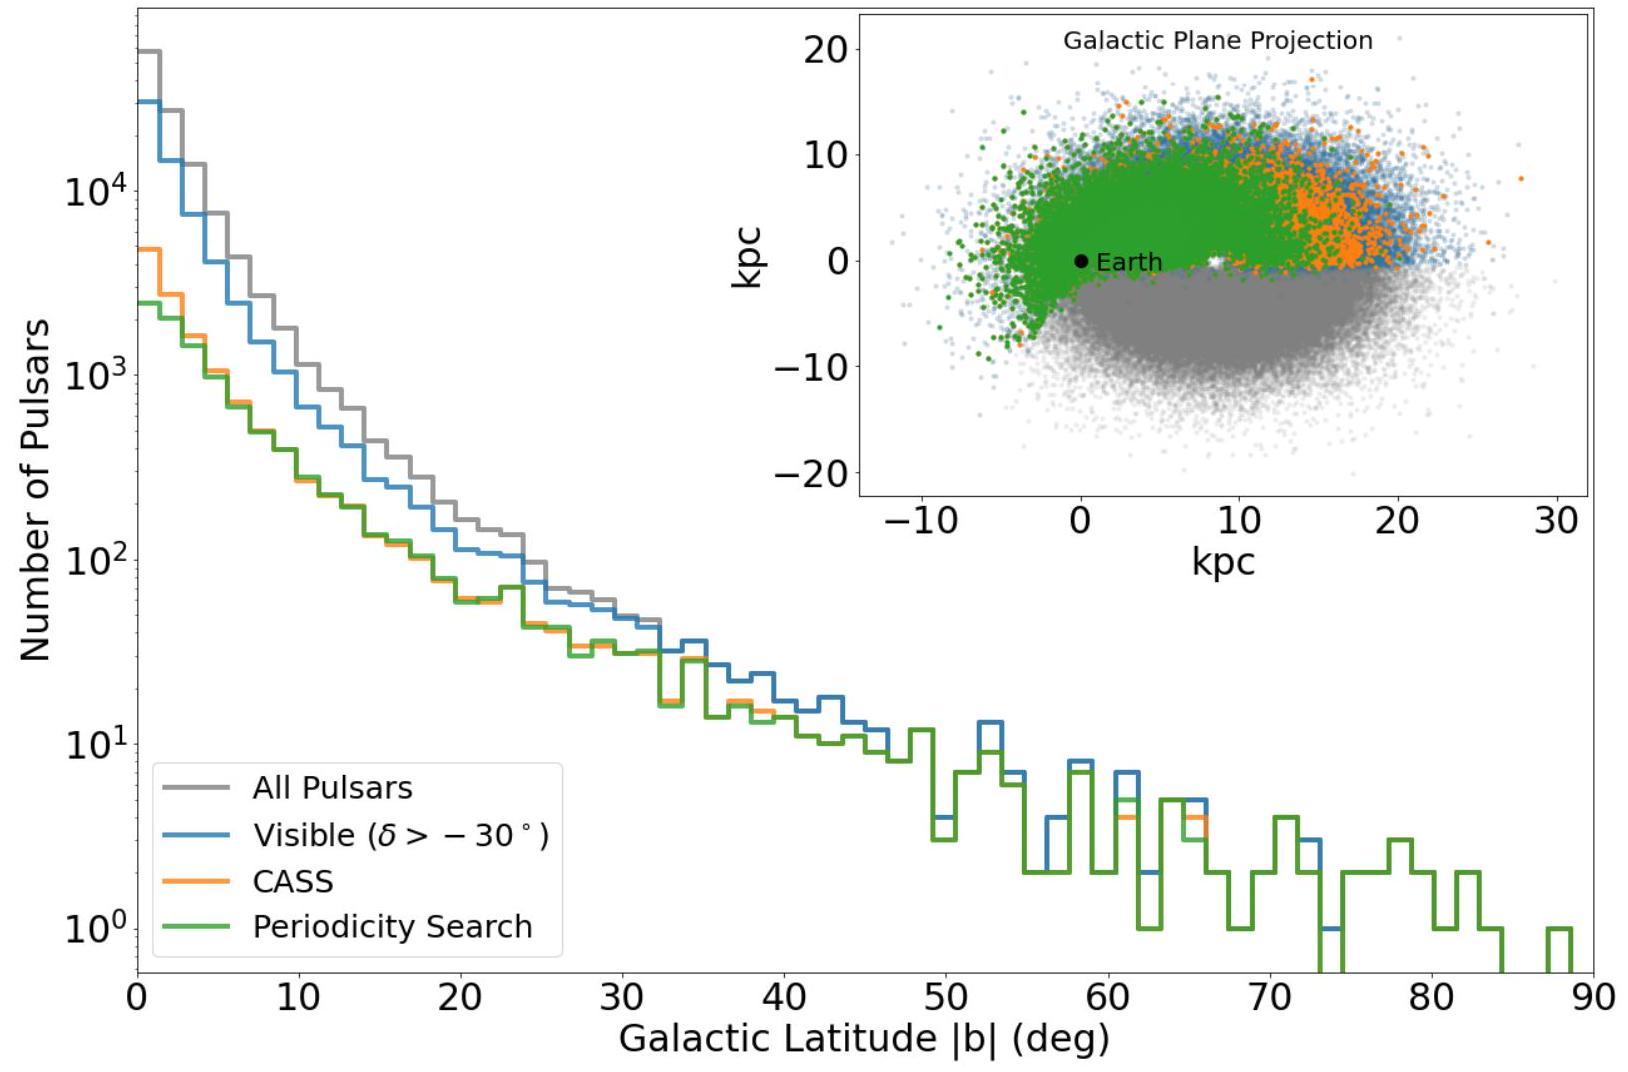
\includegraphics[width=\textwidth]{2025_09_25_a5e2be82bf0d5400f6dag-07}
\captionsetup{labelformat=empty}
\caption{Figure 1:Histogram of Galactic Latitude of Simulated Pulsar Population. The inset plot shows the population in Cartesian coordinates projected into the Galactic Plane. For both plots, the full simulated sample is in grey, the (\textbackslash delta>30\^{}\{\textbackslash circ}) population is in blue, the 25902 pulsars detectable by CASS are in orange, and the 10879 detectable by periodicity search are in green.\}\end{center}
\end{figure}

\footnotetext{\({ }^{\text {a }}\) The original \(G=4.17 \mathrm{~K} /\) Jy estimate is conservative and assumes that an arbitrary fraction of baselines would be removed to reduce computation for the pulsar search (SEFD\~{}6 Jy). The current design now assumes that all baselines will be included, leading to a significant improvement in gain ( \(G=17.5 \mathrm{~K} / \mathrm{Jy}\) ) in addition to the effect of hardware updates.
}\begin{center}
\begin{tabular}{|c|c|c|}
\hline
 & DSA-2000 Document No. 00151 & Version: 1.3 \\
\(\square S \wedge-20 \mathrm{O}\) & \begin{tabular}{c}
Pulsar Survey Forecasts and Strategies for the DSA- \\
2000 \\
\end{tabular} & \begin{tabular}{c}
Date: \(2025-09-22\) \\
Page: \(8 / 19\) \\
\end{tabular} \\
\hline
\end{tabular}
\end{center}

\begin{figure}[h]
\begin{center}
  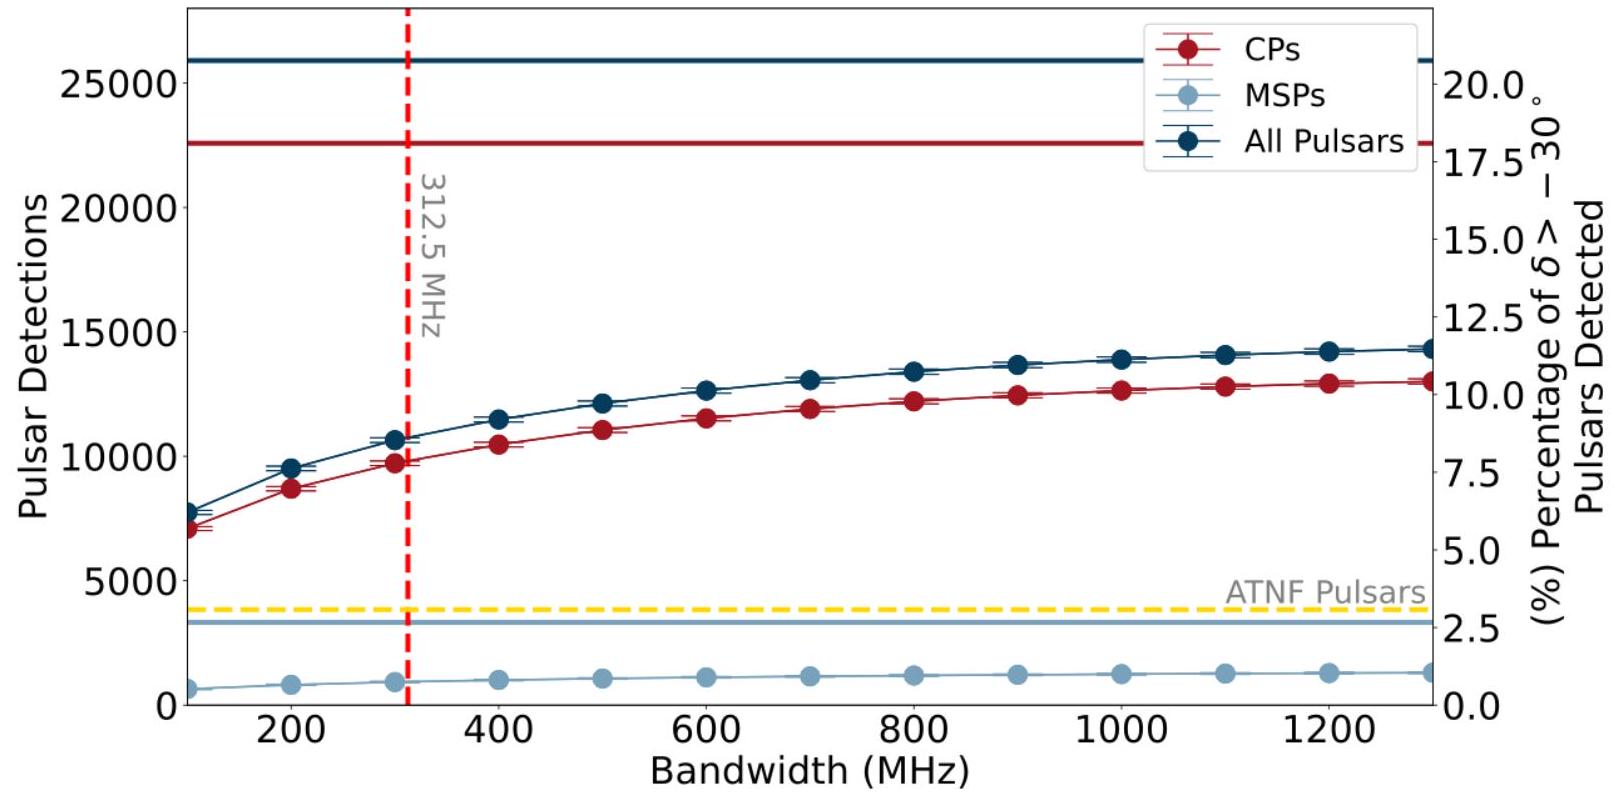
\includegraphics[width=\textwidth]{2025_09_25_a5e2be82bf0d5400f6dag-08}
\captionsetup{labelformat=empty}
\caption{Figure 2:Simulated DSA-2000 Detections from a Blind Periodicity Search as a Function of Observing Bandwidth. \(1 \sigma\) errorbars are shown. Each trial bandwidth uses 700 MHz as the lower limit; the nominal 312.5 MHz design bandwidth is indicated in red. The right-hand axis indicates the percent of the total pulsar population detected. The solid horizontal lines indicate the number of pulsars detectable in the CASS. The known pulsar population ( 3838 total) from the ATNF catalog is shown in yellow, as of May (10\^{}\{\textbackslash text \{th }\}, 2025).\}\end{center}
\end{figure}

\section*{4 CASS Target Selection and Multi-Wavelength Cross-Matching}
With the advent of rack-based GPU architectures that achieve \(\sim 100 \times\) faster compute speed ( \(\sim 10\) PFLOPS) than the current state-of-the-art and revolutionary inter-GPU data transfer rates ( \(\sim 100 \mathrm{~TB} \mathrm{~s}{ }^{-1}\) ), the DSA-2000 pulsar search will face few limitations from compute resources. This freedom may enable a full-FOV pulsar search, previously limited to only a subset of beams. Alternatively, limiting the number of search beams could enable a dense sampling of the period, DM, and acceleration parameter space. The latter case is further motivated by the expectation of \(\sim 4000\) total pulsars in each pointing, far fewer than the maximum \(\sim 10^{6}\) beams that can be formed. Over the first year of operation, the DSA-2000 CASS will build a radio image and continuum point source catalog to \(\sim 1.2 \mu \mathrm{Jy}\). In this section, we describe a potential search strategy which targets continuum sources from the initial CASS epoch to limit the number of beams. Leveraging the continuum survey will also increase the probability of detecting pulsars in the blind search and recovering faint pulsars that are not detectable in the periodicity search.

After continuum point sources are identified (details on the photometry and detection pipeline will be detailed in Akeson et al., in prep), the target selection process will generally consist of removing extended sources and cross-matching with optical and IR (OIR) galaxy catalogs. Various methods have been developed to separate resolved objects from point sources in astrophysical images, such as PSF photometry and Kron magnitude comparisons. Full-band CASS images will have a resolution \(\sim 3.02^{\prime \prime}\), enabling confident rejection of resolved false positives. Cross-matching will leverage all-sky OIR galaxy and extended source catalogs to rule out star-forming galaxies (SFGs) and active galactic nuclei (AGNs) that dominate at low flux (e.g. Condon et al. 2002). The DESI Legacy Imaging Surveys (Dey et al. 2019) and the Sloan Digital Sky Survey (SDSS; Ahumada et al. 2020) have conducted deep OIR imaging of over \(\sim 10^{5} \mathrm{deg}^{2}\) of combined extragalactic sky, producing galaxy catalogs to AB magnitudes \(\lesssim 22\). Next generation IR telescopes like the Roman (Bailey et al. 2023; Wang et al. 2022), Euclid (Scaramella et al. 2022), and SPHERE-x (Alibay et al. 2023; Feder et al. 2024) telescopes will be launched concurrently with the DSA-2000 commissioning and first light, producing catalogs of \(\sim 10^{6-8}\) galaxies imaged to \(J \lesssim 20,24.5\), \({ }^{a}\) The original \(G=4.17 \mathrm{~K} /\) Jy estimate is conservative and assumes that an arbitrary fraction of baselines would be removed to reduce computation for the pulsar search (SEFD\~{}6 Jy). The current design now assumes that all baselines will be included, leading to a significant improvement in gain ( \(G=17.5 \mathrm{~K} / \mathrm{Jy}\) ) in addition to the effect of hardware updates.

\begin{center}
\begin{tabular}{|c|c|c|}
\hline
 & DSA-2000 Document No. 00151 & Version: 1.3 \\
\(\square S \wedge-20 \mathrm{O}\) & \begin{tabular}{c}
Pulsar Survey Forecasts and Strategies for the DSA- \\
2000 \\
\end{tabular} & \begin{tabular}{c}
Date: \(2025-09-22\) \\
Page: \(9 / 19\) \\
\end{tabular} \\
\hline
\end{tabular}
\end{center}

and 26.7, respectively (Akeson et al. 2024, 2025). These data sets will be essential for any targeted search to properly select Galactic pulsar candidates and rule-out extragalactic point sources from continuum images.

As a preliminary example, consider a source selection procedure for a single \(0.63^{\circ}\) ( \(75 \% 2 \mathrm{GHz}\) PSF) pulsar search radius using a CASS continuum image and a Roman telescope source catalog. We apply a prototype source selection pipeline to a \(0.63^{\circ}\) cutout of the COSMOS deep field, one of the only sky regions observed to a similar depth, spatial resolution, and wavelength coverage as enabled by the DSA-2000 and the Roman telescopes. Let the CASS catalog be modeled by the MeerKAT international GHz Tiered Extragalactic Exploration (MIGHTEE; Jarvis et al. 2017) survey and Very Large Array COSMOS 20 cm (VLAC20; Bondi et al. 2008; Schinnerer et al. 2010, 2007) source catalogs. With source catalog thresholds \(\gtrsim 30 \mu \mathrm{Jy}\) and \(\gtrsim 6 \mu \mathrm{Jy}\), respectively, and spatial resolutions of \(5^{\prime \prime}\) and \(1.5^{\prime \prime}\), respectively, these approximate the \(3.06^{\prime \prime}\) CASS resolution and \(7 \mu \mathrm{Jy}(6 \sigma)\) detection threshold reasonably well. We approximate the Roman catalog using the Hubble Space Telescope (HST) COSMOS (Scoville et al. 2007; Leauthaud et al. 2007; Cosmos Team 2020) source catalog and the COSMOS15 (Laigle et al. 2016) galaxy catalog. The former reaches survey depth \(I \lesssim 26.5\) with \(0.12^{\prime \prime}\) resolution, while the latter reaches \(i^{+} \lesssim 26.9\) with \(\sim 0.15^{\prime \prime}\) resolution. These also compare well to the Roman I \(\lesssim 28\) OIR sensitivity and \(\sim 0.1^{\prime \prime}\) resolution.

We threshold the MIGHTEE/VLAC20 catalog at the \(7 \mu \mathrm{Jy}\) pulsar search threshold, remove sources fit with multiple Gaussian components or identified as radio galaxies in VLAC20, then cross match with HST extended sources and COSMOS15 galaxies brighter than \(I \lesssim 28\). The final sample is highlighted in red in Figure 3, demonstrating that this simple selection strategy can reduce 11537 initial continuum sources to 1901 search targets in a \(0.63^{\circ}\) radius field. Scaling the target count with the search area, we estimate the full \(0.84^{\circ}\) primary beam radius would result in \(\sim 20500\) initial sources and 3400 search targets. Notably, this example neglects the flux range from \(7-30 \mu \mathrm{Jy}\) on spatial scales from \(3.06^{\prime \prime}-5^{\prime \prime}\). Using the Condon et al. (2002) 1.4 GHz source count distributions and the Tiered Radio Extragalactic Continuum Simulation (TRECS) angular size distribution (Bonaldi et al. 2019, Figure 11), we estimate that an additional \(\sim 3200\) SFGs will be detected as unresolved point sources, while \(\sim 1400\) AGN will be detected, but ruled out as extended sources \(\left(\sim 10^{\prime \prime}\right)\). We conclude that for a pulsar search radius \(\Delta \theta\), a total sample of \(\sim 25100\left(\frac{\Delta \theta}{0.84^{\circ}}\right)^{2}\) radio continuum sources can be narrowed to \(\sim 6600\left(\frac{\Delta \theta}{0.84^{\circ}}\right)^{2}\) pulsar search targets. Incorporating other selection criteria such as polarization and spectral index, or reducing the search radius, may further narrow the selected search beams (e.g. Kaplan et al. 2019). In Section 5, we discuss how reducing the search radius will impact survey planning and follow-up.

The strategy above is intended only as a simple demo; the cross-matching strategy will be improved during design, construction, and commissioning of the DSA-2000. For example, in-development custom point source detection algorithms leverage prior knowledge of DSA-2000 systematics to minimize extended source contamination (Akeson et al., in prep.). Learning-based pipelines like the Gradient Boosting algorithm XGBoost are also upgrading the classification process (Liu et al. 2025). A more detailed investigation of source confusion's sensitivity impact with forward modeling is currently underway (Rosero et al. in prep.; Huang \& Hallinan 2022). In general, we expect confusion limits in CASS images to be wellbelow the \(7 \mu \mathrm{Jy}\) search threshold used for pulsar target selection. Naturally, source selection will be impeded within the Galactic Plane due to OIR source crowding, high interstellar extinction, diffuse radio synchrotron emission, and limited data for cross-referencing (extragalactic survey telescopes will maximize time at high Galactic latitudes). UV tapering, while effective at removing diffuse emission, introduces significant artifacts that further contaminate the source count. In Section 5, we briefly address how optimizing survey cadence can improve Galactic Plane observations, but a more rigorous study is left to future work (e.g. Faber et al., in prep). This analysis nonetheless demonstrates the efficacy of the DSA2000's unique pulsar search strategy.

\footnotetext{\({ }^{\text {a }}\) The original \(G=4.17 \mathrm{~K} /\) Jy estimate is conservative and assumes that an arbitrary fraction of baselines would be removed to reduce computation for the pulsar search (SEFD\~{}6 Jy). The current design now assumes that all baselines will be included, leading to a significant improvement in gain ( \(G=17.5 \mathrm{~K} / \mathrm{Jy}\) ) in addition to the effect of hardware updates.
}\begin{center}
\begin{tabular}{|c|c|c|}
\hline
 & DSA-2000 Document No. 00151 & Version: 1.3 \\
\(\square S \wedge-20 \mathrm{O}\) & \begin{tabular}{c}
Pulsar Survey Forecasts and Strategies for the DSA- \\
2000 \\
\end{tabular} & \begin{tabular}{c}
Date: \(2025-09-22\) \\
Page: \(10 / 19\) \\
\end{tabular} \\
\hline
\end{tabular}
\end{center}

\begin{figure}[h]
\begin{center}
  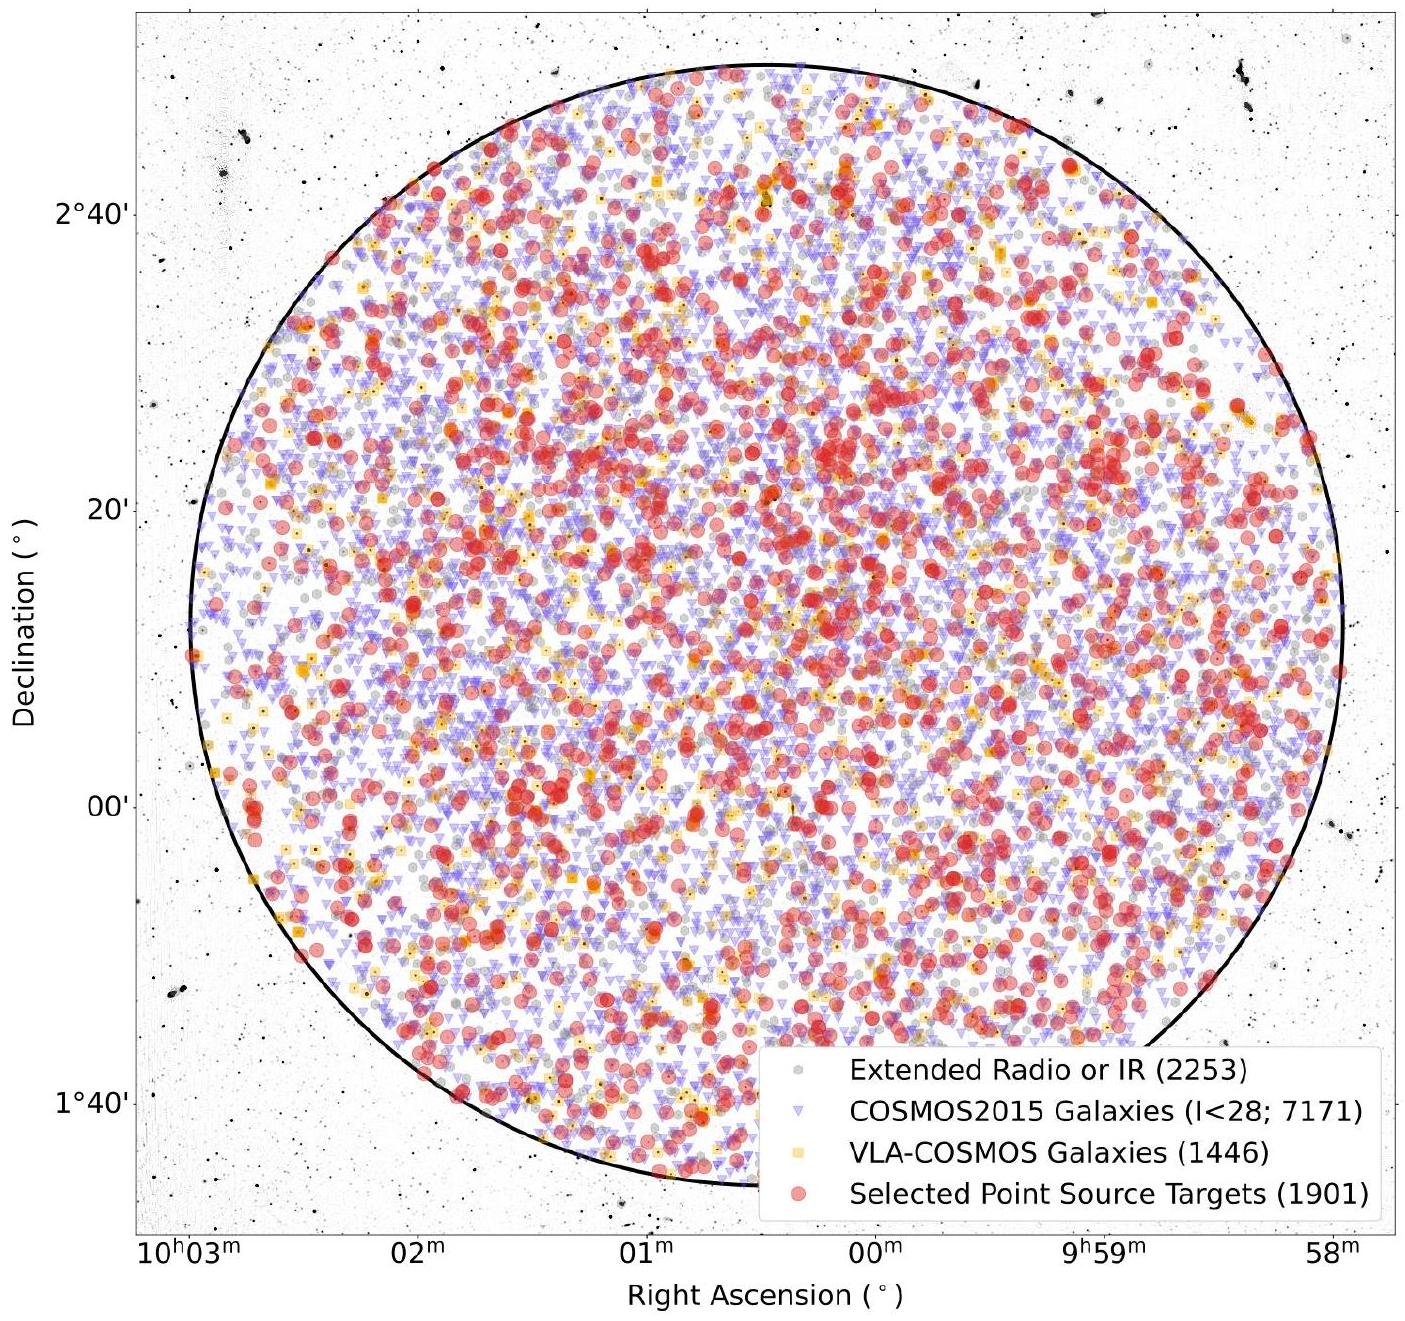
\includegraphics[width=\textwidth]{2025_09_25_a5e2be82bf0d5400f6dag-10}
\captionsetup{labelformat=empty}
\caption{Figure 3: Example Pulsar Target Selection Using the COSMOS Deep Field. The underlying image is from the MeerKAT MIGHTEE survey. MIGHTEE/VLAC20 sources excluded as extended in radio or optical are grey circles. COSMOS2015 and VLAC20 Galaxies are marked with purple triangles and orange squares, respectively. The final target sample is indicated by red circles.}
\end{center}
\end{figure}

While we have demonstrated that pulsar search targets can be selected via a robust classification and cross-matching strategy, additional source crowding and diffuse synchrotron emission motivate alternate strategies for the Galactic Plane, where most pulsars reside (see Figure 2). Fortunately, CASS pointings will be dynamically scheduled such that each search region will be visited with a flexible week-to-month cadence. By visiting the Galactic Plane more frequently (\~{}weekly), the same sensitivity of a targeted search can be recovered with randomly positioned search beams on a short timescale. Only \(\sim 30\) such epochs with

\footnotetext{\({ }^{\text {a }}\) The original \(G=4.17 \mathrm{~K} /\) Jy estimate is conservative and assumes that an arbitrary fraction of baselines would be removed to reduce computation for the pulsar search (SEFD\~{}6 Jy). The current design now assumes that all baselines will be included, leading to a significant improvement in gain ( \(G=17.5 \mathrm{~K} / \mathrm{Jy}\) ) in addition to the effect of hardware updates.
}\begin{center}
\begin{tabular}{|c|c|c|}
\hline
 & DSA-2000 Document No. 00151 & Version: 1.3 \\
\(\square S \wedge-20 \mathrm{O}\) & \begin{tabular}{c}
Pulsar Survey Forecasts and Strategies for the DSA- \\
2000 \\
\end{tabular} & \begin{tabular}{c}
Date: 2025-09-22 \\
Page: \(11 / 19\) \\
\end{tabular} \\
\hline
\end{tabular}
\end{center}

\(\lesssim 4500\) random beams each are required to sample all \(\sim 10^{5}\) continuum sources per pointing, effectively matching the targeted search sensitivity.

\section*{5 Cadence, Follow-up, and Confirmation Strategy}
By running commensally with the CASS, the pulsar search can leverage densely sampled pointings to recover sensitivity. As shown in Figure 4, CASS pointings are spaced by \(1.68^{\circ}\) in a hexagonal grid, with a minimum of 25 adjacent pointings within each scheduling block. In the current design, pulsar search beams will be confined to the \(1.68^{\circ}\) FWHM. The top plots in Figure 5 show that at low frequencies, a wider search field would allow some regions to be targeted on subsequent pointings, up to 12 times for a search field \(\theta_{p s r}=2 \theta_{P S F}\), where \(\theta_{P S F}\) is the primary beam FWHM. In these regions, one can recover the targeted search sensitivity by randomly forming beams in each pointing in only \(\sim 5\) hours as opposed to waiting for the subsequent epochs. At higher frequencies, the smaller primary beam size minimizes pointing overlap, and the targeted search remains the optimal strategy.

An effective pulsar search also requires candidates to be followed-up and confirmed on later pointings. In the current design, a subset of beams will be formed on the outer part of the primary beam to follow-up pulsar candidates. This can either be done on later epochs or, as in the case above, on adjacent pointings within the same epoch. Notably, targeting the same search beam in a subsequent pointing will have a lower sensitivity since it will be formed at a larger offset from the pointing center. The bottom plot in Figure 5 shows the cumulative sensitivity if each beam is targeted with the maximum number of adjacent pointings. At the middle of the frequency band ( 1.35 GHz ), revisiting the same beams improves the sensitivity by only a factor of 2 because they are outside of the FWHM of the adjacent beam. On the contrary, up to \(\sim 7 \times\) the on-axis sensitivity can be recovered for a small number of beams using a larger search field at low frequencies. Thus, follow-up and confirmation will be most effectively pursued by placing the tunable 312.5 MHz search band between \(700-1100 \mathrm{MHz}\).

The smaller FOV at mid- and high-frequency bands is still effective at reducing confusion from nearby continuum sources. While search beams cannot be re-visited as frequently, continuum point sources will appear narrower above 1.35 GHz due to the smaller PSF and can be more easily targeted. One potential survey strategy leveraging the full band is to run a targeted search over a single epoch at 1.35 GHz , and on the next epoch, follow-up candidates at 0.7 GHz with a larger search field. Each candidate can be observed in multiple adjacent pointings, maximizing the on-source time and increasing the chance of a re-detection for confirmation. Overlapping pulsar search fields will also have benefits for timing of known pulsars, as discussed in Liu et al. (2023); this will be investigated further in future work (Faber et al, in prep).

\footnotetext{\({ }^{\text {a }}\) The original \(G=4.17\) K/Jy estimate is conservative and assumes that an arbitrary fraction of baselines would be removed to reduce computation for the pulsar search (SEFD\~{}6 Jy). The current design now assumes that all baselines will be included, leading to a significant improvement in gain ( \(G=17.5 \mathrm{~K} / \mathrm{Jy}\) ) in addition to the effect of hardware updates.
}\begin{center}
\begin{tabular}{|c|c|c|}
\hline
 & DSA-2000 Document No. 00151 & Version: 1.3 \\
\(\square S \wedge-20 \mathrm{O}\) & \begin{tabular}{c}
Pulsar Survey Forecasts and Strategies for the DSA- \\
2000 \\
\end{tabular} & \begin{tabular}{c}
Date: 2025-09-22 \\
Page: \(12 / 19\) \\
\end{tabular} \\
\hline
\end{tabular}
\end{center}

\begin{figure}[h]
\begin{center}
  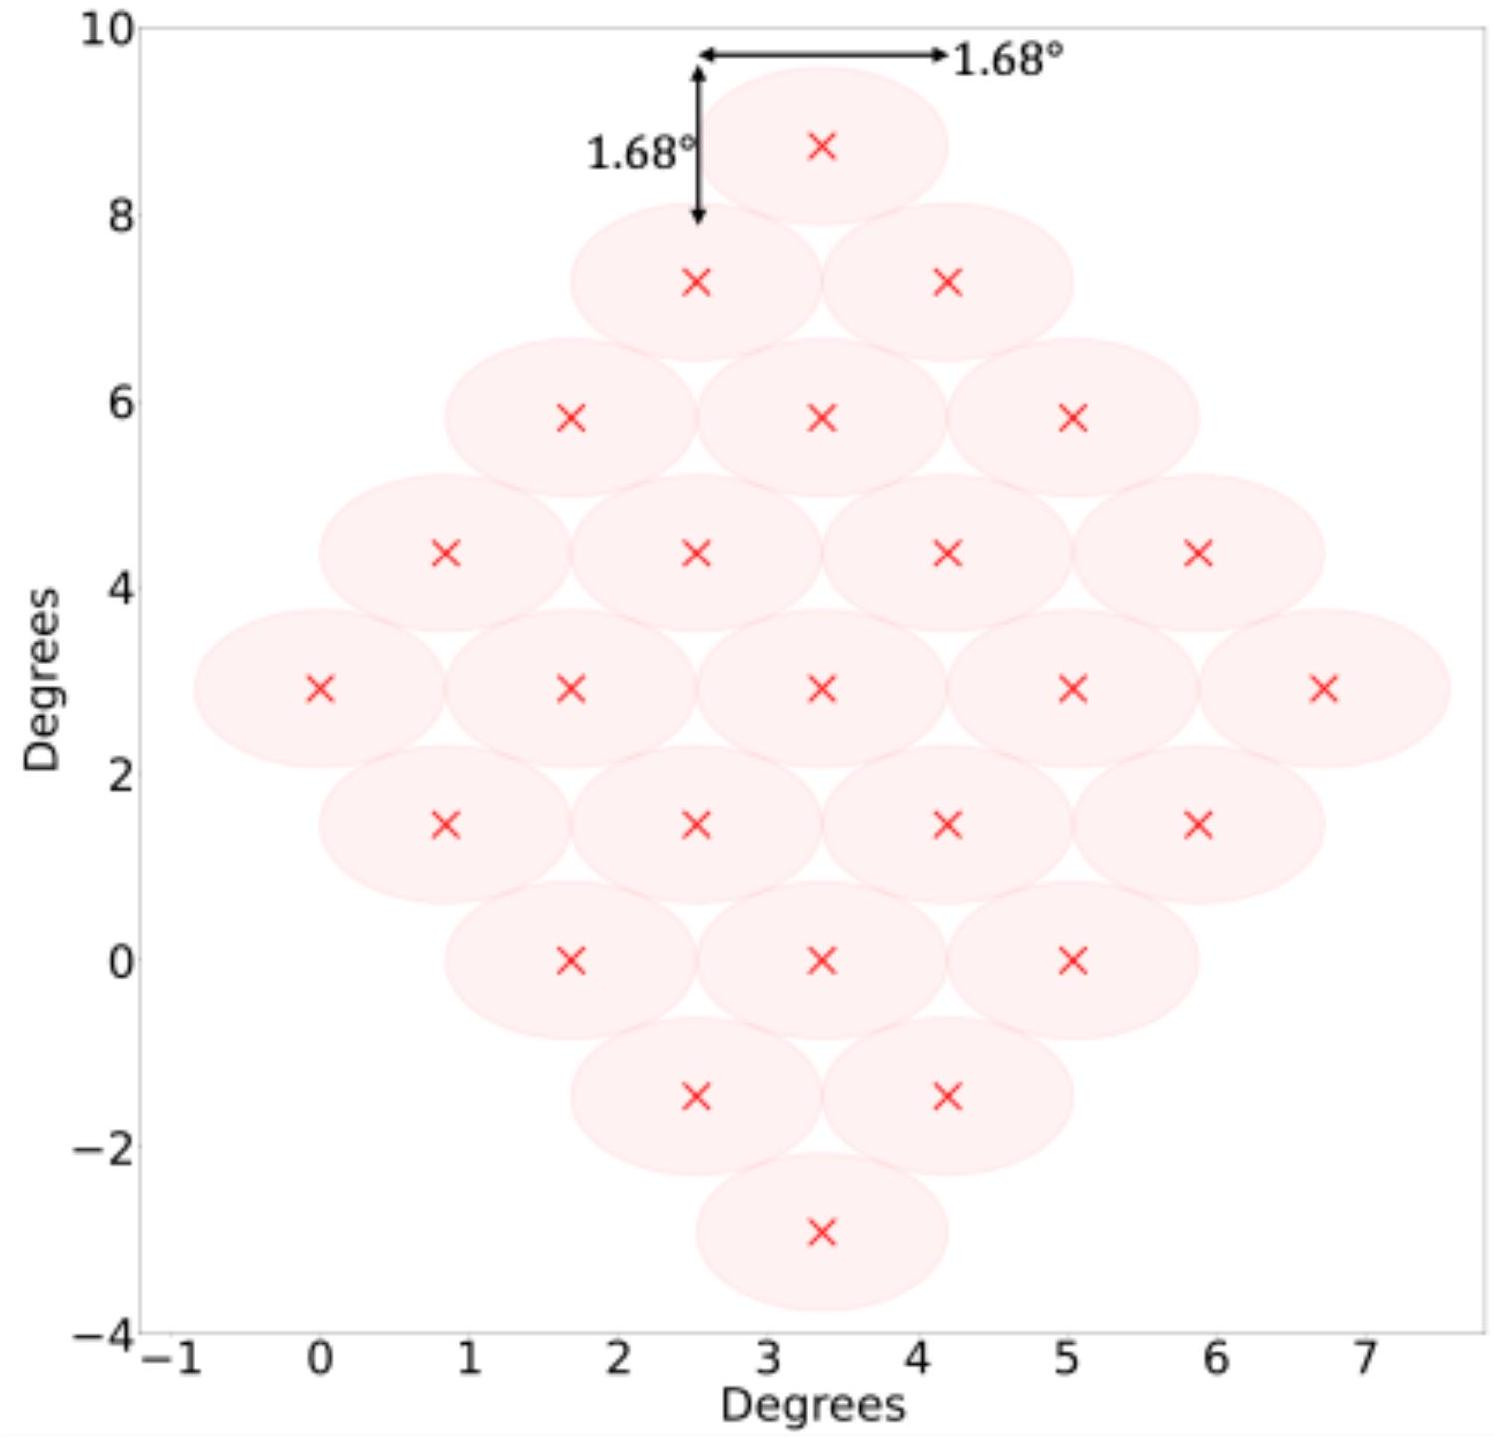
\includegraphics[width=\textwidth]{2025_09_25_a5e2be82bf0d5400f6dag-12}
\captionsetup{labelformat=empty}
\caption{Figure 4: Example 25-Pointing Grid for DSA-2000 CASS. Pointing centers are indicated by an "x", and each circle indicates the FWHM of the primary beam at (2 \textbackslash mathrm\{GHz}\textbackslash left(1.68\^{}\{\textbackslash circ\}\textbackslash right)).\}\end{center}
\end{figure}

\footnotetext{\({ }^{\text {a }}\) The original \(G=4.17\) K/Jy estimate is conservative and assumes that an arbitrary fraction of baselines would be removed to reduce computation for the pulsar search (SEFD\~{}6 Jy). The current design now assumes that all baselines will be included, leading to a significant improvement in gain ( \(G=17.5 \mathrm{~K} / \mathrm{Jy}\) ) in addition to the effect of hardware updates.
}\begin{center}
\begin{tabular}{|c|c|c|}
\hline
 & DSA-2000 Document No. 00151 & Version: 1.3 \\
\(\square S \wedge-20 \mathrm{O}\) & \begin{tabular}{c}
Pulsar Survey Forecasts and Strategies for the DSA- \\
2000 \\
\end{tabular} & \begin{tabular}{c}
Date: 2025-09-22 \\
Page: 13/19 \\
\end{tabular} \\
\hline
\end{tabular}
\end{center}

\begin{figure}[h]
\begin{center}
  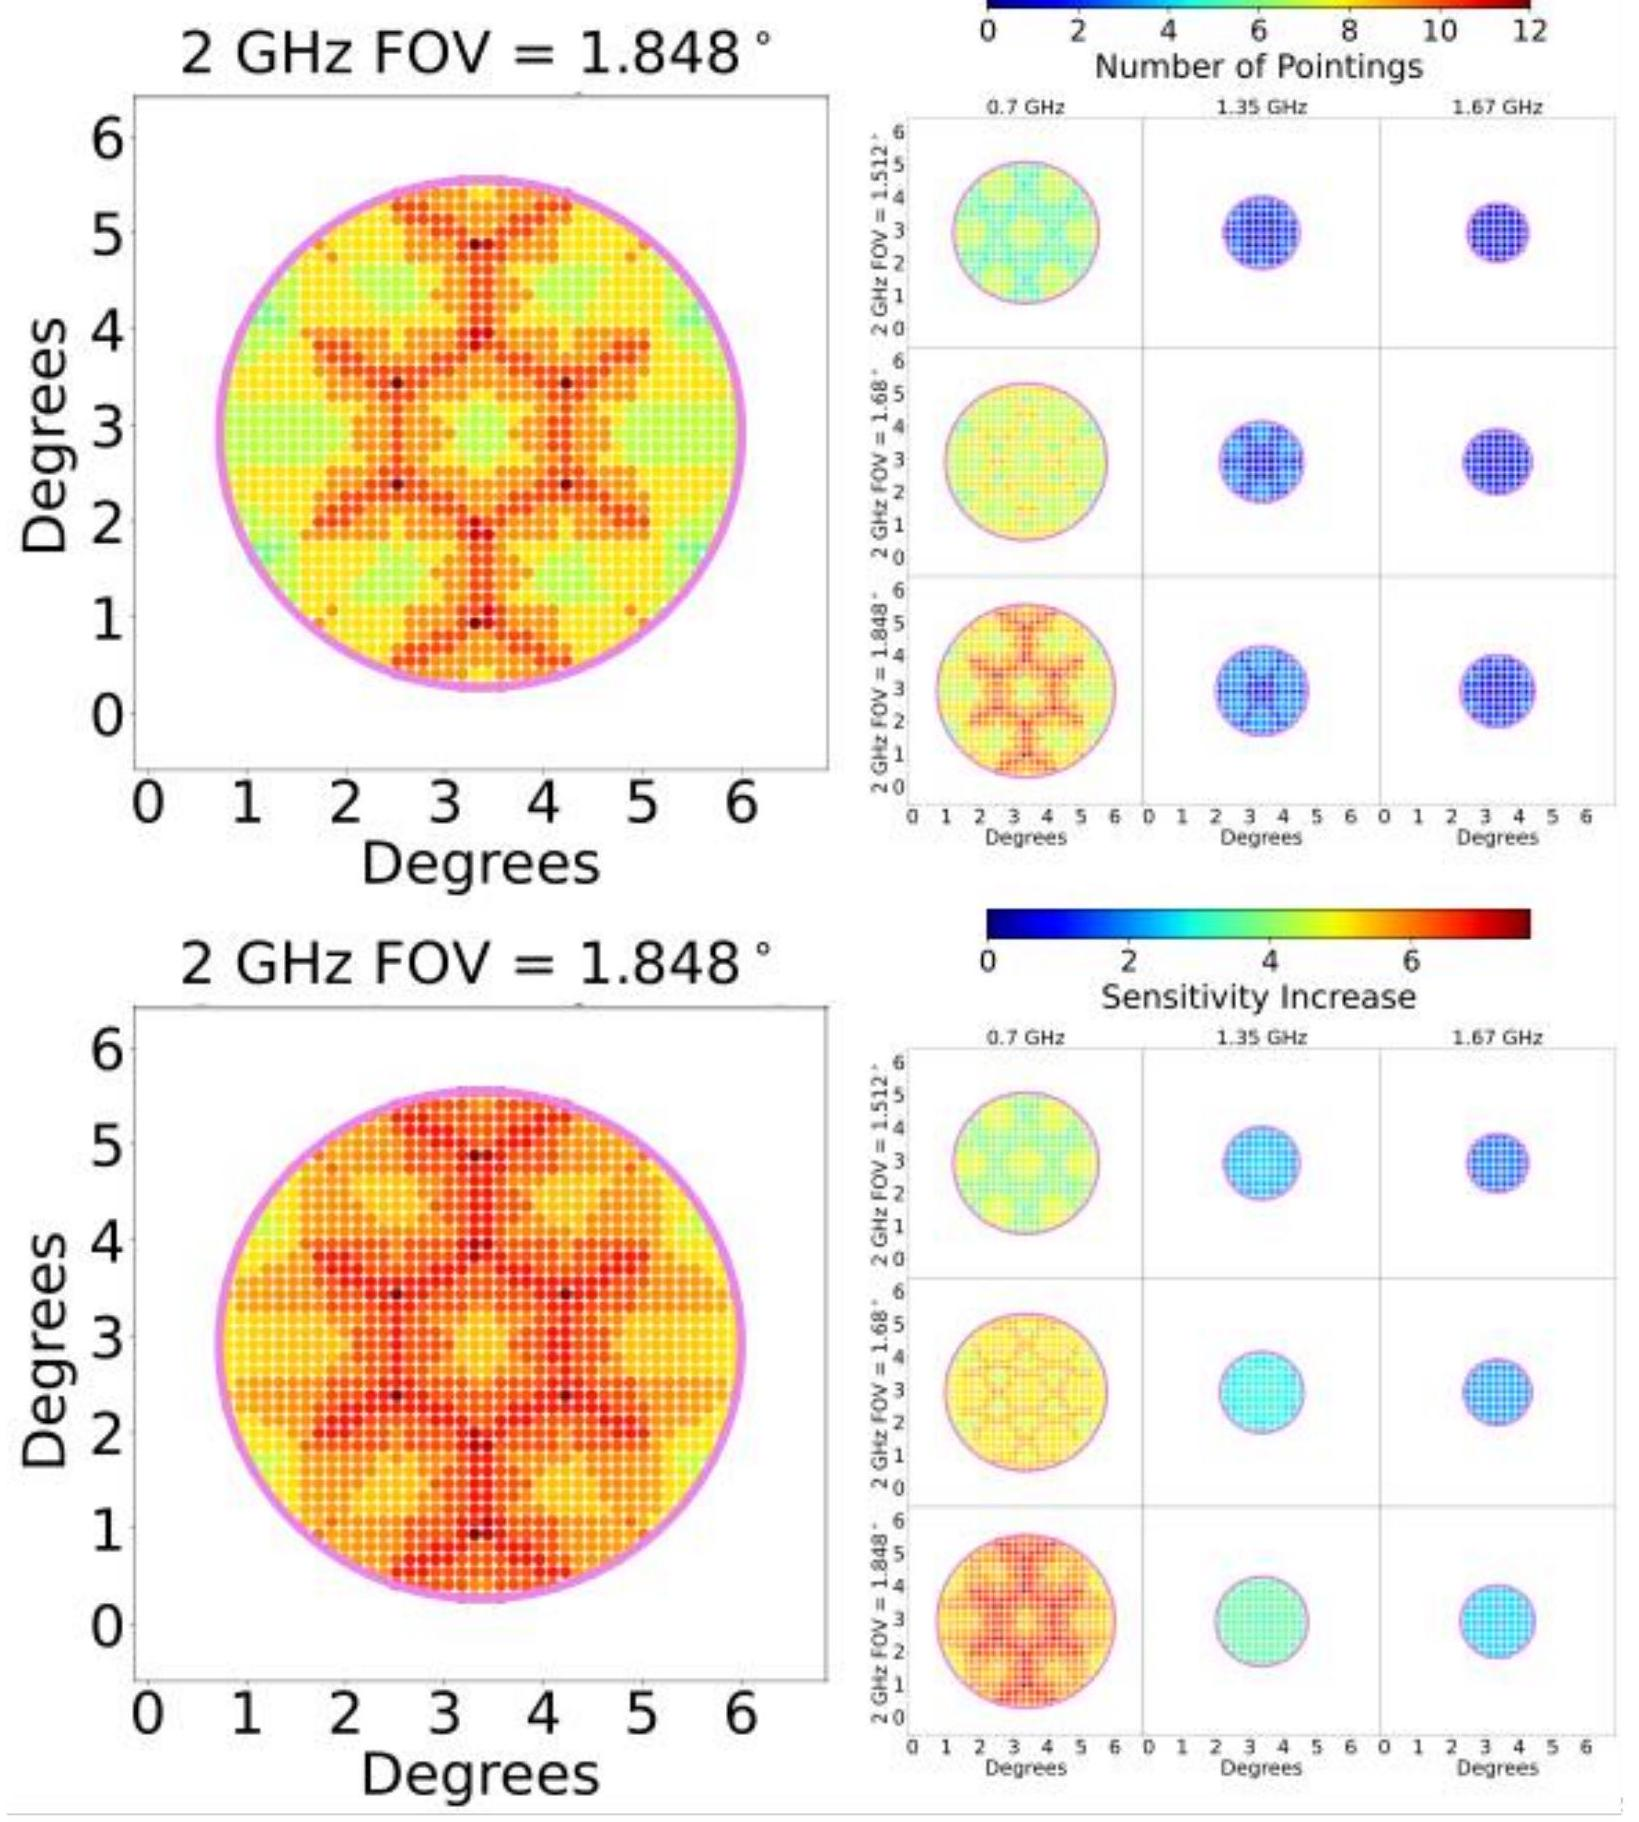
\includegraphics[width=\textwidth]{2025_09_25_a5e2be82bf0d5400f6dag-13}
\captionsetup{labelformat=empty}
\caption{Figure 5: (top right) Number of adjacent pointings that overlap each point within example pulsar search FOVs. Each row corresponds to a different search region size and each column corresponds to a different frequency band. The pink circle indicates the edge of the search region, while the colorscale indicates the number of times a point can be visited within a 25 -pointing grid. (bottom right) Sensitivity increase factor from re-visiting a point the maximum number of times. The rows and columns are identical to the bottom left plot. The top left and bottom left plots are zoomed in on the (\textbackslash mathrm\{FOV}=1.848\^{}\{\textbackslash circ\}) example.\}\end{center}
\end{figure}

\footnotetext{\({ }^{\text {a }}\) The original \(G=4.17 \mathrm{~K} /\) Jy estimate is conservative and assumes that an arbitrary fraction of baselines would be removed to reduce computation for the pulsar search (SEFD\~{}6 Jy). The current design now assumes that all baselines will be included, leading to a significant improvement in gain ( \(G=17.5 \mathrm{~K} / \mathrm{Jy}\) ) in addition to the effect of hardware updates.
}\begin{center}
\begin{tabular}{|c|c|c|}
\hline
 & DSA-2000 Document No. 00151 & Version: 1.3 \\
\(\square S \wedge-20 \mathrm{O}\) & \begin{tabular}{c}
Pulsar Survey Forecasts and Strategies for the DSA- \\
2000 \\
\end{tabular} & \begin{tabular}{c}
Date: 2025-09-22 \\
Page: \(14 / 19\) \\
\end{tabular} \\
\hline
\end{tabular}
\end{center}

\section*{6 Conclusion}
In this memo, we have considered the prospects for a DSA-2000 pulsar search, proposed a possible continuum source targeting strategy, and considered ways to optimize follow-up given the overlapping CASS pointing design. We have demonstrated that while the blind pulsar search will detect \(\sim 10^{4}\) pulsars, sensitivity can be improved by targeting continuum sources from the CASS, extending the forecasted detections to \(\sim 3000\) MSPs and \(\sim 20000\) CPs. Overlapping adjacent pointings at low frequencies will enable rapid follow-up of candidates. Future work will investigate the DSA-2000's sensitivity to exotic, high acceleration pulsar binaries, and discuss the Generic-GPU-Project FTD search system in detail. With a flexible FTD architecture and unique search strategies, the DSA-2000 will make a lasting contribution to pulsar science, enabling population studies that will characterize their progenitors and probe intervening matter.

\section*{7 Appendix: Modelling the Effective DSA-2000 Blind Search S/N Threshold}
General practice for pulsar detection forecasting is to assume a constant S/N threshold, S/N \({ }_{\min } \approx 9\) (e.g. Cordes et al. 2006). However, Lazarus et al. (2015) use injection tests of Arecibo Pulsar-ALFA Survey (PALFA) pipeline to demonstrate that \(\mathrm{S} / \mathrm{N}_{\min }\) cannot be fully described by the radiometer equation, especially at low pulse periods. Biases in the search algorithm can affect \(\mathrm{S} / \mathrm{N}_{\text {min }}\) resulting in over-estimated pulsar detection predictions. It is essential to understand the baseline search performance, as future efforts will incorporate novel GPU-based optimization. To this end, a Monte Carlo simulation was conducted to characterize the true \(\mathrm{S} / \mathrm{N}_{\min }\) as a function of the FFT size M , the pulse period P , and the sampling rate \(\mathrm{t}_{\mathrm{s}}\). The method described follows a similar procedure to Smith (2016) to analyze novel search algorithms. For a given trial FFT size, a Monte Carlo simulation was conducted by generating a population of pulsar timeseries with randomly selected pulse periods \(\mathrm{P}, \mathrm{S} / \mathrm{N}\), and duty cycle (estimated as \(\mathrm{D}=1 / \mathrm{n}_{\text {harms }}\) ) drawn from uniform distributions ranging from \(0.1 \mathrm{~Hz} \leq 1 / \mathrm{P} \leq 1000 \mathrm{~Hz}\) (note here that the distribution is uniform in frequency rather than period for better interfacing with the algorithm) and \(0 \leq \mathrm{S} / \mathrm{N} \leq 100\). Each timeseries is assumed to have radiometer noise RMS given by:

\[
\sigma=\frac{T_{\text {sys }}}{\sqrt{2 \Delta f t_{\text {int }}}}
\]

where \(\mathrm{T}_{\text {sys }}, \Delta f\), and \(\mathrm{t}_{\text {int }}\) are the system temperature, channel bandwidth, and integration time. For simplicity, the effects of scintillation, scattering, and dispersion were neglected. The generated pulsar was then assumed to be a perfectly de-dispersed timeseries averaged over frequency. Future work will involve incorporating more realistic effects (such as scintillation and scattering) into trial pulsars.

Each pulsar was then run through a prototype Python implementation of a power spectrum folding search, which takes as parameters the maximum number of harmonics to fold, \(\mathrm{n}_{\text {folds }}\), and an FFT size M. This is identical to a standard pulsar folding algorithm but sums only harmonics of the pulse period, which is known a-priori. A "detection" is defined as the case where the maximum search statistic \(\widehat{\varepsilon}_{\text {max }}\) exceeds a critical threshold \(\eta\), such that the probability of the search statistic exceeding \(\eta\) is:

\[
P\left(\hat{\varepsilon}_{\max }>\eta\right)=N_{\text {trials }}^{-1}=\left(N_{D M}\left(M t_{s}\left(f_{\max }-f_{\min }\right)\right) N_{s k y}\right)^{-1}
\]

where the number of trials \(\mathrm{N}_{\text {trials }}\) is the total number of trials, including frequency trials \(\left(M t_{s}\left(f_{\text {max }}-f_{\text {min }}\right)\right)\), DM trials, and sky pointings. A histogram versus input S/N of each pulsar is created for total pulsars \(H_{\text {tot }}(S / N)\) and detected pulsars \(H_{\text {det }}(S / N)\), binning by \(\Delta \mathrm{S} / \mathrm{N}=1\), and the detection probability taken to be the ratio:

\[
P_{\operatorname{det}}(S / N)=\frac{H_{\operatorname{det}}(S / N)}{H_{t o t}(S / N)}
\]

\footnotetext{\({ }^{\text {a }}\) The original \(G=4.17 \mathrm{~K} /\) Jy estimate is conservative and assumes that an arbitrary fraction of baselines would be removed to reduce computation for the pulsar search (SEFD\~{}6 Jy). The current design now assumes that all baselines will be included, leading to a significant improvement in gain ( \(G=17.5 \mathrm{~K} / \mathrm{Jy}\) ) in addition to the effect of hardware updates.
}\begin{center}
\begin{tabular}{|c|c|c|}
\hline
 & DSA-2000 Document No. 00151 & Version: 1.3 \\
\(\square S \wedge-20 \mathrm{O}\) & \begin{tabular}{c}
Pulsar Survey Forecasts and Strategies for the DSA- \\
2000 \\
\end{tabular} & \begin{tabular}{c}
Date: 2025-09-22 \\
Page: \(15 / 19\) \\
\end{tabular} \\
\hline
\end{tabular}
\end{center}

as shown in Figure 6 (top). The \(\mathrm{S} / \mathrm{N}\) threshold estimate \(\mathrm{S} / \mathrm{N}_{\text {min }}\) is defined to be where \(P_{\text {det }}\left(S / N_{\text {min }}\right)=0.5\) after fitting a non-central \(\chi^{2}\) distribution.

The resulting S/N threshold as a function of pulse frequency is shown in Figure 6 (bottom) for 0.1 ms sampling time and \(\mathrm{M}=9 \times 10^{6} . \mathrm{S} / \mathrm{N}_{\mathrm{min}}\) is approximately constant with average value \(\mathrm{S} / \mathrm{N}_{\mathrm{min}, \text { avg }}=9.4 \sigma\). This suggests that the DSA-2000 search's high time resolution and sensitivity make it relatively robust against period-dependent effects, such as red noise (e.g. Singh et al. 2022), though a more detailed analysis is required to confirm this. \(\mathrm{S} / \mathrm{N}_{\min }\) is extrapolated and applied to \href{http://PSRPop.py}{PSRPop.py} by re-calculating the beamaveraged \(\mathrm{S} / \mathrm{N}\) for each pulsar and comparing it the \(\mathrm{S} / \mathrm{N}_{\text {min }}\) for the given pulse period. Figure 7 shows the revised detectable pulsar population compared to the original \(9 \sigma\) threshold sensitivity curves. The impact of the revised threshold is most prominent for MSPs with DM \(\gtrsim 200 \mathrm{pc} \mathrm{cm}^{-3}\), reducing the MSP blind search forecast by \(\sim 12 \%\), while CP detections are reduced by \(\sim 8 \%\). This effect is incorporated into the uncertainties reported in Section 3 for the blind search predictions.

\footnotetext{\({ }^{\text {a }}\) The original \(G=4.17\) K/Jy estimate is conservative and assumes that an arbitrary fraction of baselines would be removed to reduce computation for the pulsar search (SEFD\~{}6 Jy). The current design now assumes that all baselines will be included, leading to a significant improvement in gain ( \(G=17.5 \mathrm{~K} / \mathrm{Jy}\) ) in addition to the effect of hardware updates.
}\begin{center}
\begin{tabular}{|c|c|c|}
\hline
 & DSA-2000 Document No. 00151 & Version: 1.3 \\
\(\square S \wedge-20 \mathrm{O}\) & \begin{tabular}{c}
Pulsar Survey Forecasts and Strategies for the DSA- \\
2000 \\
\end{tabular} & \begin{tabular}{c}
Date: 2025-09-22 \\
Page: \(16 / 19\) \\
\end{tabular} \\
\hline
\end{tabular}
\end{center}

\begin{figure}[h]
\begin{center}
  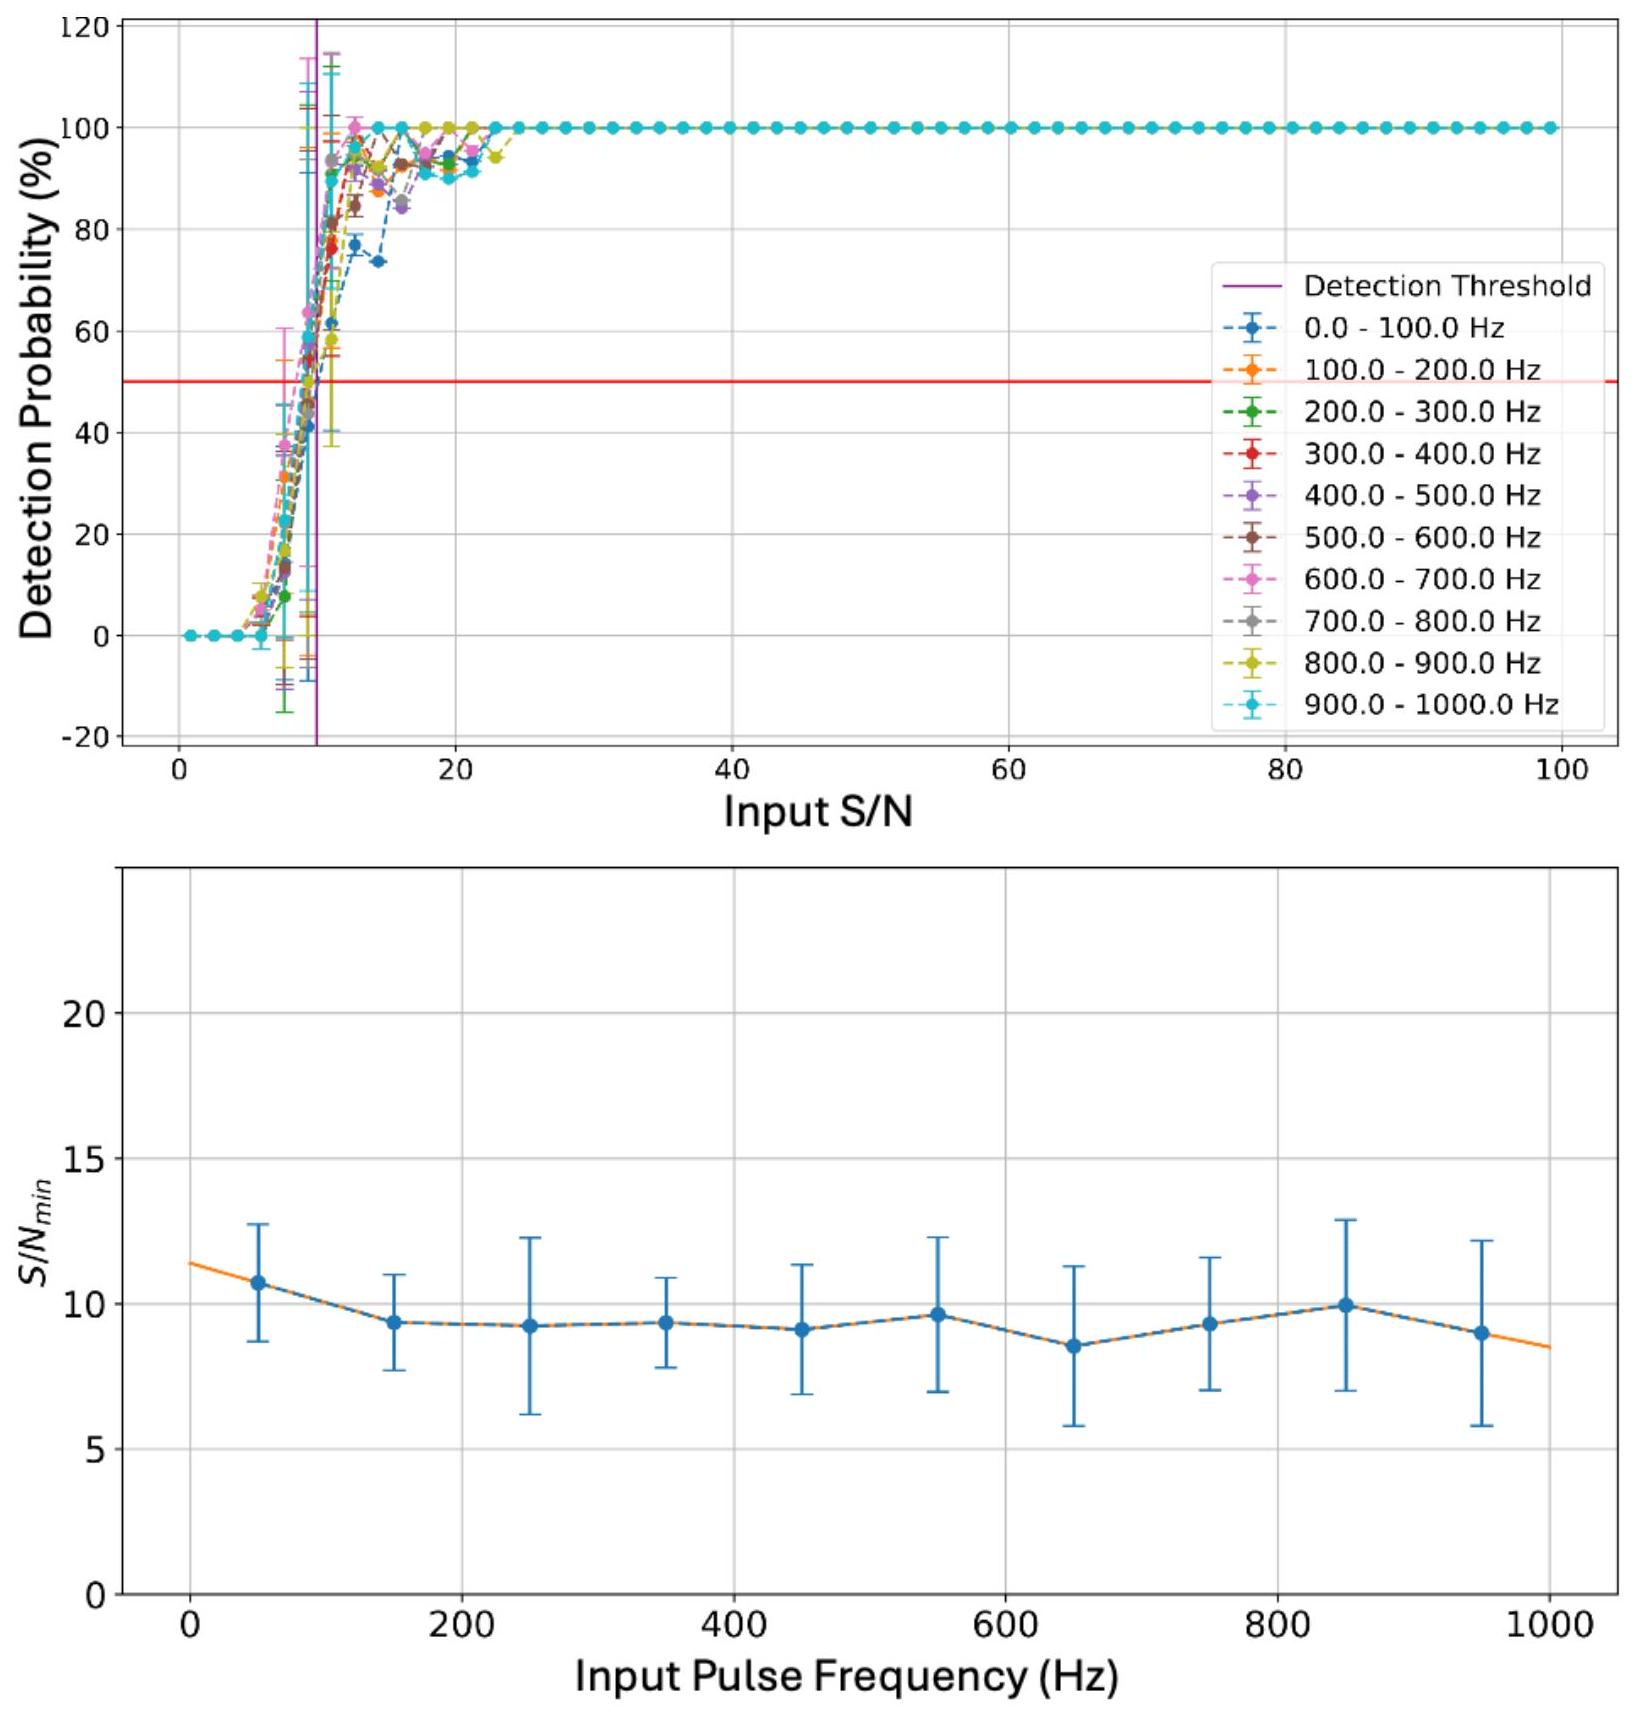
\includegraphics[width=\textwidth]{2025_09_25_a5e2be82bf0d5400f6dag-16}
\captionsetup{labelformat=empty}
\caption{Figure 6: (top) Detection Probability Curves for the Baseline Search. The red line indicates the \(50 \%\) detection probability corresponding to the S/N threshold. The purple line indicates the threshold \(\eta\) set by the false positive rate \(\alpha\) used as the detection criteria on the search statistic. (bottom) S/N Threshold for Baseline Search. Linear interpolation is shown as a solid line, which is used for constraint of PSRPop.py simulations.}
\end{center}
\end{figure}

\footnotetext{\({ }^{\text {a }}\) The original \(G=4.17 \mathrm{~K} /\) Jy estimate is conservative and assumes that an arbitrary fraction of baselines would be removed to reduce computation for the pulsar search (SEFD\~{}6 Jy). The current design now assumes that all baselines will be included, leading to a significant improvement in gain ( \(G=17.5 \mathrm{~K} / \mathrm{Jy}\) ) in addition to the effect of hardware updates.
}\begin{center}
\begin{tabular}{|c|c|c|}
\hline
 & DSA-2000 Document No. 00151 & Version: 1.3 \\
\(\square S \wedge-20 \mathrm{O}\) & \begin{tabular}{c}
Pulsar Survey Forecasts and Strategies for the DSA- \\
2000 \\
\end{tabular} & \begin{tabular}{c}
Date: 2025-09-22 \\
Page: \(17 / 19\) \\
\end{tabular} \\
\hline
\end{tabular}
\end{center}

\begin{figure}[h]
\begin{center}
  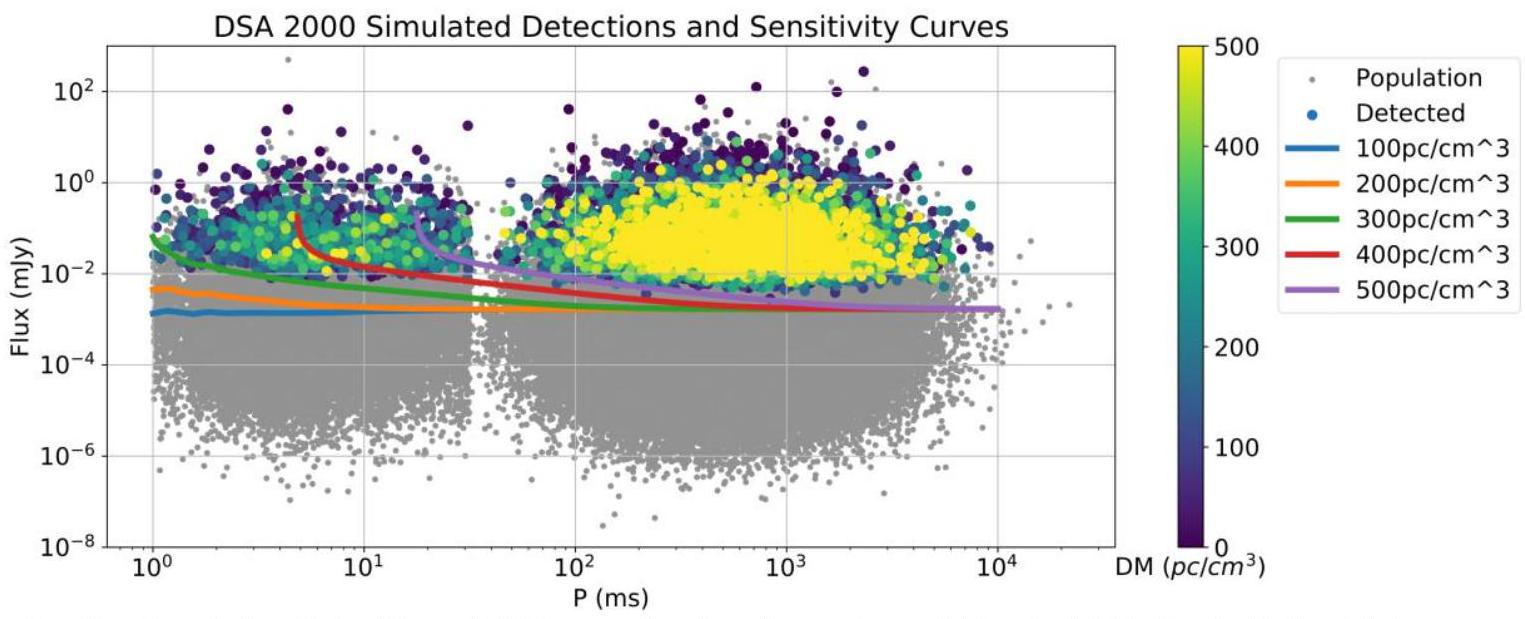
\includegraphics[width=\textwidth]{2025_09_25_a5e2be82bf0d5400f6dag-17}
\captionsetup{labelformat=empty}
\caption{Figure 7: Baseline Search Sensitivity Plot and PSRPop.py Simulated Detections with Revised S/N Threshold. Sensitivity curves with the original constant (\textbackslash mathrm\{S} / \textbackslash mathrm\{N\}) threshold of 9 are shown as solid lines.\}\end{center}
\end{figure}

\section*{8 References}
Ahumada, R., Allende Prieto, C., Almeida, A., et al. 2020, ApJS, 249, 3\\
Akeson, R., Armus, L., Desai, V., et al. 2024in, 261-08\\
Akeson, R. et al. 2025, in American Astronomical Society Meeting Abstracts, Vol. 245, 131-06\\
Alibay, F., Sindiy, O. V., Jansma, P. T., et al. 2023, in 2023 IEEE Aerospace Conference, IEEE, 1-18\\
Amiri, M., Andersen, B. C., Bandura, K., et al. 2021, The Astrophysical Journal Supplement Series, 257, 59

Amiri, M., Bandura, K., Boskovic, A., et al. 2022, The Astrophysical Journal Supplement Series, 261, 29

Backer, D. \& Hellings, R. 1986, Annual review of astronomy and astrophysics, 24, 537\\
Bailes, M., Jameson, A., Abbate, F., et al. 2020, Publications of the Astronomical Society of Australia, 37, e028

Bailey, V. P., Bendek, E., Monacelli, B., et al. 2023, Techniques and Instrumentation for Detection of Exoplanets XI, 12680, 283

Barr, E. D., Champion, D. J., Kramer, M., et al. 2013, Monthly Notices of the Royal Astronomical Society, 435, 2234

Bates, S., Lorimer, D., Rane, A., \& Swiggum, J. 2014, Monthly Notices of the Royal Astronomical Society, 439, 2893

Bhattacharyya, B., Cooper, S., Malenta, M., et al. 2016, The Astrophysical Journal, 817, 130\\
Bonaldi, A., Bonato, M., Galluzzi, V., et al. 2019, Monthly Notices of the Royal Astronomical Society, 482, 2

Bondi, M., Ciliegi, P., Schinnerer, E., et al. 2008, The Astrophysical Journal, 681, 1129\\
Condon, J., Cotton, W., \& Broderick, J. 2002, The Astronomical Journal, 124, 675\\
Cordes, J. M., Freire, P. C. C., Lorimer, D. R., et al. 2006, ApJ, 637, 446\\
Cordes, J. M. \& Lazio, T. J. W. 2002, arXiv preprint astro-ph/0207156\\
Cosmos Team. 2020, COSMOS ACS I-band Photometry Catalog, NASA IPAC DataSet, IRSA169\\
Dey, A., Schlegel, D. J., Lang, D., et al. 2019, AJ, 157, 168\\
Dimoudi, S., Adamek, K., Thiagaraj, P., et al. 2018, The Astrophysical Journal Supplement Series, 239, 28

Dong, F. A., Crowter, K., Meyers, B. W., et al. 2023, Monthly Notices of the Royal Astronomical Society, 524, 5132

\footnotetext{\({ }^{\text {a }}\) The original \(G=4.17 \mathrm{~K} /\) Jy estimate is conservative and assumes that an arbitrary fraction of baselines would be removed to reduce computation for the pulsar search (SEFD\~{}6 Jy). The current design now assumes that all baselines will be included, leading to a significant improvement in gain ( \(G=17.5 \mathrm{~K} / \mathrm{Jy}\) ) in addition to the effect of hardware updates.
}\begin{center}
\begin{tabular}{|c|c|c|}
\hline
 & DSA-2000 Document No. 00151 & Version: 1.3 \\
\(\square S \wedge-20 \mathrm{O}\) & \begin{tabular}{c}
Pulsar Survey Forecasts and Strategies for the DSA- \\
2000 \\
\end{tabular} & \begin{tabular}{c}
Date: \(2025-09-22\) \\
Page: \(18 / 19\) \\
\end{tabular} \\
\hline
\end{tabular}
\end{center}

Eatough, R. P., Kramer, M., Lyne, A., \& Keith, M. 2013, Monthly Notices of the Royal Astronomical Society, 431, 292

Edwards, R., Bailes, M., van Straten, W., \& Britton, M. 2001, Monthly Notices of the Royal Astronomical Society, 326, 358

Feder, R. M., Masters, D. C., Lee, B., et al. 2024, The Astrophysical Journal, 972, 68\\
Fruchter, A., Stinebring, D., \& Taylor, J. 1988, Nature, 333, 237\\
Hallinan, G., Ravi, V., Weinreb, S., et al. 2019, in Bulletin of the American Astronomical Society, Vol. 51, 255

Haslam, G., Wielebinski, R., \& Priester, W. 1982, Sky and Telescope, 63, 230\\
Huang, Y. \& Hallinan, G. 2022, in American Astronomical Society Meeting Abstracts, Vol. 240, American Astronomical Society Meeting \#240, 314.06

Jarvis, M. J., Taylor, A., Agudo, I., et al. 2017, arXiv preprint arXiv:1709.01901\\
Kaplan, D. L., Dai, S., Lenc, E., et al. 2019, The Astrophysical Journal, 884, 96\\
Keith, M., Jameson, A., van Straten, W., et al. 2010, Monthly Notices of the Royal Astronomical Society, 409, 619

Laigle, C., McCracken, H. J., Ilbert, O., et al. 2016, The Astrophysical Journal Supplement Series, 224, 24

Lattimer, J. M. 2012, Annual Review of Nuclear and Particle Science, 62, 485\\
Law, C. J., Sharma, K., Ravi, V., et al. 2023, arXiv preprint arXiv:2307.03344\\
Lazarus, P., Brazier, A., Hessels, J., et al. 2015, The Astrophysical Journal, 812,81\\
Leauthaud, A., Massey, R., Kneib, J.-P., et al. 2007, The Astrophysical Journal Supplement Series, 172, 219

Liu, C., Miller, A. A., Bloom, J. S., Knop, R. A., \& Nugent, P. E. 2025, AMorphological Model to Separate Resolved-unresolved Sources in the DESI Legacy Surveys: Application in the LS4 Alert Stream

Liu, T., Cohen, T., McGrath, C., Demorest, P. B., \& Vigeland, S. J. 2023, The Astrophysical Journal, 945, 78

Manchester, R., Lyne, A., Taylor, J., et al. 1978, Monthly Notices of the Royal Astronomical Society, 185, 409

Manchester, R. N., Hobbs, G. B., Teoh, A., \& Hobbs, M. 2005, The Astronomical Journal, 129, 1993\\
Manchester, R. N., Lyne, A., d'Amico, N., et al. 1996, Monthly Notices of the Royal Astronomical Society, 279, 1235

Manchester, R. N., Lyne, A. G., Camilo, F., et al. 2001, Monthly Notices of the Royal Astronomical Society, 328, 17

Men, Y., Barr, E., Clark, C. J., Carli, E., \& Desvignes, G. 2023, Astronomy \& Astrophysics, 679, A20

Ng, C., Champion, D., Bailes, M., et al. 2015, Monthly Notices of the Royal Astronomical Society, 450, 2922

Ng, C., Wu, B., Ma, M., et al. 2020, The Astrophysical Journal, 903, 81\\
Radhakrishnan, V. \& Cooke, D. 1969\\
Ransom, S. M., Eikenberry, S. S., \& Middleditch, J. 2002, The Astronomical Journal, 124, 1788\\
Ravi, V., Catha, M., Chen, G., et al. 2023, The Astrophysical Journal Letters, 949, L3\\
Roberts, M. S., Search, F. P., \& Collaborations, G. D. S. S. 2011 in, American Institute of Physics, 127-130

Scaramella, R., Amiaux, J., Mellier, Y., et al. 2022, Astronomy \& Astrophysics, 662, A112\\
Schinnerer, E., Sargent, M., Bondi, M., et al. 2010, The Astrophysical Journal Supplement Series, 188, 384

Schinnerer, E., Smoľ ci' c, V., Carilli, C., et al. 2007, The Astrophysical Journal Supplement Series, 172, 46

Scoville, N., Abraham, R., Aussel, H., et al. 2007, The Astrophysical Journal Supplement Series, 172, 38\\
\({ }^{\text {a }}\) The original \(G=4.17 \mathrm{~K} /\) Jy estimate is conservative and assumes that an arbitrary fraction of baselines would be removed to reduce computation for the pulsar search (SEFD\~{}6 Jy). The current design now assumes that all baselines will be included, leading to a significant improvement in gain ( \(G=17.5 \mathrm{~K} / \mathrm{Jy}\) ) in addition to the effect of hardware updates.

\begin{center}
\begin{tabular}{|c|c|c|}
\hline
 & DSA-2000 Document No. 00151 & Version: 1.3 \\
\(\square S \wedge-20 \mathrm{O}\) & \begin{tabular}{c}
Pulsar Survey Forecasts and Strategies for the DSA- \\
2000 \\
\end{tabular} & \begin{tabular}{c}
Date: 2025-09-22 \\
Page: \(19 / 19\) \\
\end{tabular} \\
\hline
\end{tabular}
\end{center}

Sharma, K., Ravi, V., Connor, L., et al. 2024, Nature, 635, 61\\
Singh, S., Roy, J., Panda, U., et al. 2022, The Astrophysical Journal, 934, 138\\
Smith, K. M. 2016, arXiv preprint arXiv:1610.06831\\
Smits, R., Kramer, M., Stappers, B., et al. 2009, Astronomy \& Astrophysics, 493, 1161\\
Spitler, L., Cordes, J. M., Hessels, J., et al. 2014, The Astrophysical Journal, 790, 101\\
Stovall, K., Lynch, R., Ransom, S., et al. 2014, The Astrophysical Journal, 791, 67\\
Thongmeearkom, T., Clark, C., Breton, R., et al. 2024, Monthly Notices of the Royal Astronomical Society, 530, 4676\\
van der Wateren, E., Bassa, C. G., Cooper, S., et al. 2023, Astronomy \& Astrophysics, 669, A160\\
van Haarlem, M. P., Wise, M. W., Gunst, A., et al. 2013, Astronomy \& Astrophysics, 556, A2\\
Wang, Y., Zhai, Z., Alavi, A., et al. 2022, The Astrophysical Journal, 928, 1\\
Weltman, A., Bull, P., Camera, S., et al. 2020, Publications of the Astronomical Society of Australia, 37, e002

\footnotetext{\({ }^{\text {a }}\) The original \(G=4.17\) K/Jy estimate is conservative and assumes that an arbitrary fraction of baselines would be removed to reduce computation for the pulsar search (SEFD\~{}6 Jy). The current design now assumes that all baselines will be included, leading to a significant improvement in gain ( \(G=17.5 \mathrm{~K} / \mathrm{Jy}\) ) in addition to the effect of hardware updates.
}
\end{document}